\documentclass[journal]{IEEEtran}
\usepackage[T1]{fontenc}
\usepackage[utf8]{inputenc}
\usepackage{amsmath,amssymb}
\usepackage{graphicx}
\usepackage{booktabs}
\usepackage{multirow}
\usepackage{xcolor}
\usepackage[colorlinks=true,linkcolor=blue,citecolor=blue,urlcolor=blue]{hyperref}
\hyphenation{op-tical net-works semi-conduc-tor}
\begin{document}

\title{Front matter}

\author{Ali~Hosseini$^{*}$, and Saeed~Sedighi%
\thanks{Manuscript submitted to the IEEE Journal of Oceanic Engineering.%
The authors are with the Department of Computer Engineering, Shiraz
Branch (Shi.C.), Islamic Azad University, Shiraz, Iran.%
$^{*}$Corresponding author: Ali Hosseini
(e-mail: ali.hosseini7148@iau.ac.ir; saeed.sedighi@iau.ac.ir).}}

\markboth{IEEE Journal of Oceanic Engineering}%
{Hosseini and Sedighi: PhysINR-Zero}

\IEEEtitleabstractindextext{%
\begin{abstract}
Underwater imaging supports civilian ocean engineering --- inspection, environmental monitoring, marine robotics --- yet enhancement methods are hard to compare, and the strongest supervised ones need paired training data a new site cannot supply. We present PhysINR-Zero, an enhancement method that carries no underwater training data, and evaluate it with HydroBench, a protocol that re-runs every method under one implementation, one split and one metric set. PhysINR-Zero represents the scene as a coordinate field of physical quantities --- per-channel optical thickness, a bounded nonlinear correction and ambient light --- inverting a Jerlov-based forward model. Its 10,296 parameters are meta-trained on synthetic degradations of terrestrial photographs by first-order MAML, then adapted to each image against reference-free losses, then rendered through a reference-free display stage that restores the contrast the conservative inverse leaves in the frame. Across 519 images from five benchmark sets against ten baselines it trails the supervised leaders by 4.5--6.6 dB PSNR on the paired sets, while ranking first of eleven on the no-reference UCIQE measure on four of the five sets --- and the two families disagree for a measurable reason: UICM, the colour-measure term of UCIQE, rewards chroma spread, the very signal a colour cast carries. The method delivers perceptual quality without signal reconstruction, on metrics the field distrusts, and the paper quantifies where that trust should end.
\end{abstract}
\begin{IEEEkeywords}
Underwater image enhancement; zero-shot learning; physics-informed neural network; test-time adaptation; image quality assessment; benchmarking
\end{IEEEkeywords}}

\section{Introduction}
Underwater imagery is the primary sensing modality for civilian ocean engineering: hull and infrastructure inspection, environmental monitoring, seafloor mapping and the perception stack of autonomous underwater vehicles. All of these degrade the image in the same way, because water attenuates light selectively by wavelength and scatters it toward the camera. The result is a colour cast toward blue-green, reduced contrast and a veiling backscatter that removes exactly the texture an inspector or a detector needs. Enhancement before analysis is not optional on most field imagery.

Two families of method address it. Supervised deep networks --- Water-Net \cite{li2020uieb}, FUnIE-GAN \cite{islam2020funie}, U-Shape Transformer \cite{peng2023ushape} --- learn the correction from paired degraded/clean images. The comparison also covers UIEC$^{2}$-Net \cite{wang2021uiec2}, Five A+ \cite{jiang2023fivea}, TOPAL \cite{jiang2022topal}, WF-Diff \cite{zhao2024wfdiff} and WaterMamba \cite{guan2024watermamba}. They recover reference structure well, and they bind to the data they were trained on: a network trained on one water type, one camera and one depth range is being applied to a different one. The classical priors --- the underwater dark channel prior \cite{drews2013udcp} and multi-scale Retinex \cite{jobson1997msr} --- need no training data and generalise anywhere, but reconstruct reference structure poorly (\S{}4.2). Between the two there is an operating point that is easy to state and hard to reach: a method that learns, but not from underwater photographs.

The second problem is measurement. Published results in this field are not comparable across papers, and the spread is not marginal. Re-runs of Water-Net on UIEB by papers that cite it span 16.305 to 19.81 dB --- a 2.8 dB range, wider than the improvement most new methods claim over their predecessor. U-Shape Transformer is credited with UIEB PSNR 21.25, 22.91 and 21.55 by three different papers. Thirty-seven such contradictions were catalogued across recent surveys, and on no-reference metrics the disagreement is proportionally worse: one method's UIQM on the same test set differs by a factor of 1.5 to 1.9 between two 2026 surveys. The causes are structural, not careless. Test populations differ --- UIEB alone is variously used as its 90 paired images, its 60-image challenge subset, a 190-image or a 45-image selection; LSUI is split 3879/400 by one group, 504 test images by another, 427 by a third. Metric implementations are re-written per paper and preprocessing varies from 256 $\times$ 256 resize to full resolution. The field has reached this conclusion independently: the comprehensive survey of Cong et al.~\cite{cong2024survey} re-ran seventeen methods under a single protocol for exactly this reason, and GuidedHybSensUIR \cite{guo2025guidedhyb} re-benchmarked thirty-seven. Any claim about a new method's standing therefore has to be made on a protocol that fixes all three: split, implementation and metric set.

This paper asks two questions and answers both empirically. Can a method that has seen no underwater photograph at all be competitive on standard benchmarks? And where, precisely, does it fall short? The answer to the second question turns out to be more interesting than the first, because the method fails predictably, in one metric family and not the other, and the failure pattern is traceable to the loss it optimises. The venue framing matters here. Benchmark and enhancement work published in the ocean-engineering literature has long treated measurement protocol as part of the method --- from the underwater image formation model of McGlamery~\cite{mcglamery1980} to the quality measures of Panetta et al.~\cite{panetta2016uiqm} and the enhancement benchmarks of Panetta et al.~\cite{panetta2022uwtbench} and Zhang et al.~\cite{zhang2022attenuated} in the IEEE Journal of Oceanic Engineering. This paper continues that convention: the protocol is specified, provenance-labelled and audited before any method is compared under it.

We present PhysINR-Zero, an enhancement method whose learned weights are meta-trained on synthetic degradations of ordinary terrestrial photographs and applied to underwater images without further training. The scene is represented as a coordinate field of physical quantities --- per-channel optical thickness, a bounded nonlinear intensity correction and ambient light --- which inverts a forward model built on the Jerlov water-type classification. At test time the field is adapted to each image against reference-free losses; the method never loads a reference image, and the code path is structured so that it cannot. The model carries 10,296 parameters.

The contributions are:

1. \textbf{A zero-shot physics-constrained enhancement method.} PhysINR-Zero    meta-trains on synthetic degradations sampled from the same forward operator    it inverts, so task distribution and inductive bias are matched by    construction. The zero-shot boundary is enforced in code, not assumed: the    training CLI refuses a source directory that resolves inside any benchmark    dataset, and a perceptual-hash deduplication pass drops near-duplicate    training sources against every evaluation split, with the counts written to    the run's provenance record. 2. \textbf{A leakage-guarded re-benchmarking protocol.} Every method in the    comparison --- classical prior, GAN, transformer and state-space model --- is    scored by one code path on five benchmark sets (519 test images) with eleven    metrics, split-disjointness verified against sha256 manifests and a table    rendered only when the columns are paired. Three baselines whose published    weights were initially unavailable were recovered to their released models    rather than left as approximations; the one method whose checkpoint cannot be    obtained is marked as a fallback and excluded from the ranking, rather than    reported as its own result. 3. \textbf{A measured split between perceptual quality and signal reconstruction.}    PhysINR-Zero trails the supervised leaders by 4.5--6.6 dB PSNR on the    paired sets, while improving on every full-reference metric relative to an    earlier prior of its own design. A reference-free display stage stretches    the conservative inverse's compressed output ranges, which moves the    no-reference colour measures to the top of the field --- first of eleven on    UCIQE on four of the five sets --- while the paired metrics keep their    ordering. The split follows the loss    terms, and a CIELAB fidelity panel against the reference photographs shows    the no-reference metrics rewarding the chroma spread that a colour cast    \emph{is} --- a result about the evaluation protocol as much as about the method. 4. \textbf{A bounded negative result.} Of fifteen ablation variants, twelve are    statistically indistinguishable from the full model on both metric    families. Three register on the no-reference side only --- colour-balance    removal and the two adaptation-length ends move UCIQE significantly --- and    exactly one, five adaptation steps, also moves PSNR detectably, costing    0.91 dB while buying 0.59 of UCIQE. That bounds the individual    contribution of the physics and regularisation loss groups rather than    establishing that they are unnecessary, and it locates the significant    variation in colour handling and adaptation budget rather than in    reconstruction.

The honest summary is in \S{}5: measured against supervised baselines on paired benchmarks, PhysINR-Zero is a perceptual-quality method rather than a signal-reconstruction method, and the no-reference metrics that rank it well are themselves distrusted by the field, including by the authors of the benchmark that supplies its test images. Both halves of that sentence are reported.


\section{Related work}
\subsection{Supervised underwater image enhancement}
The supervised family learns the mapping from degraded to clean images from paired data. Water-Net \cite{li2020uieb} introduced it together with the UIEB dataset, using a colour-estimation module and an attention-driven colour-correction network. FUnIE-GAN \cite{islam2020funie} targeted real-time deployment on robots with a conditional GAN and its own EUVP dataset. U-Shape Transformer \cite{peng2023ushape} introduced the LSUI dataset and a channel-attention U-Net variant. UIEC$^{2}$-Net \cite{wang2021uiec2} fuses features in RGB and LAB. Five A+ \cite{jiang2023fivea} demonstrated that 9K parameters suffice for competitive enhancement, which matters for embedded ocean platforms. TOPAL \cite{jiang2022topal} uses a target-oriented perceptual adversarial fusion. Diffusion entered the field with WF-Diff \cite{zhao2024wfdiff}, and the state-space models followed with WaterMamba \cite{guan2024watermamba}. Recent methods continue upward in reported accuracy: UniUIR \cite{zhang2025uniuir} reports 25.11 dB PSNR on UIEB, WWE-UIE \cite{cheng2026wweuie} 24.32 dB and Phaseformer \cite{khan2025phaseformer} 25.98 dB. Each reports under splits that none of them share, which is the comparability problem of \S{}1 quantified at the top of the reporting distribution.

\subsection{Physics-based and zero-shot methods}
The classical alternatives assume no training data. Retinex theory \cite{jobson1997msr} decomposes the image into illumination and reflectance and rescales the former; multi-scale Retinex with colour restoration remains a standard reference point. The underwater dark channel prior \cite{drews2013udcp} adapts dark-channel dehazing to wavelength-selective attenuation. Both generalise to any water body and both rank near the bottom of the paired-set metrics (\S{}4.2, Tables~\\ref{tab:uieb},~\\ref{tab:lsui},~\\ref{tab:euvp}) --- Retinex reaches 15.099 dB PSNR on UIEB against 23.654 for UIEC$^{2}$-Net --- while Retinex' strong UCIQE shows that reconstructing the reference and scoring well perceptually are different tasks.

PhysINR-Zero sits between the families. It is trained, but on synthetic degradations of terrestrial photographs, so the zero-shot boundary is with respect to real underwater data rather than with respect to training per se. Two design choices separate it from the classical priors: the water-type prior is \emph{soft} --- the field emits a distribution over the ten Jerlov types rather than committing to one --- and the adaptation is per-image, which is what lets a single initialisation serve turbid coastal water and clear oceanic water.

\subsection{Coordinate networks and test-time adaptation}
Coordinate neural networks represent a scene as a function of position. In low-level vision they are used mostly for implicit scene representation; the application here is different --- the coordinate field carries \emph{physical} quantities sampled at the image grid, not colour. Test-time adaptation through meta-learning follows first-order MAML \cite{finn2017maml}, which trades the second-order gradient of full MAML for a first-order approximation at a substantial runtime saving.

\subsection{Benchmark and protocol work}
The comparability problem has produced two kinds of response. The first is the re-run: Cong et al.~\cite{cong2024survey} re-ran seventeen methods under one protocol ''to prevent differences in metric values caused by different toolboxes or implementations'', unifying the split ratio and the metric code; Guo et al.~\cite{guo2025guidedhyb} re-benchmarked thirty-seven methods on a mixed test pool. The second is the metric critique. Li and Cavallaro~\cite{li2022limits} conclude that ''none of the no-reference quality measures satisfactorily rates the quality of enhanced underwater images'', analysing UIQM, UCIQE and CCF directly. Yang and Sowmya~\cite{yang2015uciqe} --- whose UCIQE definition this paper uses --- and Panetta et al.~\cite{panetta2016uiqm} --- whose UIQM definition it uses --- supplied the measures that later work came to dispute. WWE-UIE \cite{cheng2026wweuie} drops UIQM in favour of NIQE. The colour-cast diagnostic this benchmark reports alongside them is an internal HSV saturation measure, not one of the published measures under critique. Most directly, the UIEB benchmark paper itself states ''We discard the non-reference metrics designed for underwater image enhancement'' \cite{li2020uieb} , \S{}IV. HydroBench follows the re-benchmarking response and inherits the critique: it implements both families of metric with stated conventions, and the no-reference orderings in \S{}4.2 are read with the field's own reservations.


\section{Materials and methods}
\subsection{Physical forward model}
The method inverts a forward model of underwater image formation (\cite{mcglamery1980}; Fig.~\\ref{fig:method}). For channel \emph{c} of a pixel, the model is

\begin{align}
J_{c} = \mathrm{bounded\_{nonlinear}}(I_{c}, \alpha _{c})\label{eq:1} \\
I'_{c} = J_{c} \cdot  t_{c} + A_{c} \cdot  (1 - t_{c}) + r_{c}\label{eq:2} \\
t_{c} = \exp(-\tau _{c})\label{eq:3} 
\end{align}
where \emph{J} is the scene radiance after a bounded nonlinear correction, \emph{$\tau$} is the optical thickness per channel, \emph{A} the ambient (backscatter) light level and \emph{r} a residual. The corrected radiance is recovered by inverting \eqref{eq:2}:

\begin{align}
\hat{J}_{c} = (I_{c} - \hat{A}_{c} \cdot  (1 - \hat{t}_{c})) / (\hat{t}_{c} + \varepsilon ).\label{eq:4} 
\end{align}
The nonlinear correction in \eqref{eq:1} uses the monotone remap \emph{g(v) = v(1$-$v)(2v$-$1)} bounded by $\alpha$ $\in$ [0, 2] with a soft shoulder, which compresses recovered radiance that falls outside the displayable range back into it without clipping. The optical thickness is anchored to a water-type prior. Ten Jerlov water types \cite{jerlov1976} , Table XXVII supply a per-channel diffuse attenuation coefficient $\beta_c$, giving a prior of $\beta_c$ $\cdot$ \emph{d} for a global depth \emph{d}. The field may deviate from it by at most $\delta_{\max}$ = 1.5 in optical thickness, through a tanh activation, so the correction is bounded, smooth and saturating rather than free. The oceanic type-I row of Jerlov's table lies below pure-seawater attenuation at 9 of 15 tabulated wavelengths, which is not physically possible for a natural water body. That row is substituted with the pure-seawater attenuation curve of Austin and Petzold~\cite{austin1986kd}, the standard reference for clear oceanic $K_d$. The remaining nine rows are used as published, and the 1976 edition is used throughout --- the widely reproduced 1968 table differs from it by up to 34 \% in individual entries, and the two editions must not be mixed.

\textbf{The largest acknowledged physical approximation.} Each camera channel is read at one representative wavelength --- 608, 545 and 455 nm for R, G and B --- rather than integrating the channel's spectral response against the attenuation spectrum. The wavelengths are the peaks of each sRGB channel's response, computed from the CIE 1931 colour-matching functions and the IEC 61966-2-1 primaries under D65, so the single-point estimator weights the broadband response where it is heaviest. A broadband spectral integration would be more accurate, but it requires auxiliary spectral measurement that the method deliberately does not assume it has: it must work on ordinary sRGB imagery. This approximation is stated here rather than buried in implementation, because it is the one place the physics is weakest for exactly the channel that matters most in turbid coastal water.

\subsection{The transmission prior: level and ratio}
The prior's \textbf{spectral ratio} and its \textbf{level} are estimated by separate mechanisms, because they have different identifiability. Image formation is affine in the scene radiance, so the ambient wash shifts the image without compressing it:

\begin{align}
\mathrm{range}(I_{c}) = t_{c} \cdot  \mathrm{range}(J_{c}).\label{eq:5} 
\end{align}
The per-channel percentile range (1st--99th) therefore recovers the transmission \emph{ratios} directly,

\begin{align}
t_{\mathrm{data},c} = \mathrm{range}_{c} / \max_{c} \mathrm{range}_{c}',      \tau _{data},c = -\ln t_{\mathrm{data},c}\label{eq:6} 
\end{align}
with the least-attenuated channel as the scene reference, a 0.25 floor on the reference, and $t_{\mathrm{data}}$ = 1 when the frame carries no contrast at all. The estimator is parameter-free and needs no water type. On synthetic tasks the correlation between $\tau_{\mathrm{data}}$ and the true per-channel $\tau$ is 0.42--0.52, and the mean error in the recovered ratio is 0.05 --- the ratio is well identified.

The \textbf{level} is not. The range identity \eqref{eq:5} is scale-free: it fixes $t_{R}$ : $t_{G}$ : $t_{B}$ but leaves the common scale undetermined, and no single-frame statistic identifies it. On the UIEB test set the correlation between every image statistic examined and the true best-channel transmission is only $-$0.33 to $-$0.40, and the normalisation in \eqref{eq:6} forces the best channel to t = 1 by construction where the real value averages 0.59. An estimator-only prior therefore under-amplifies by $\approx$ 1.7$\times$ on every frame --- a deficit adaptation cannot correct, because the wrong constant is written into the prior and the inner loop has no signal to correct it against.

The level is instead \textbf{learned}, and supervised on the synthetic task's own ground truth. A linear head on the same 41-dimensional content descriptor as the water-type head predicts the best-channel transmission, and the outer meta-loop supervises it against the sampled task's own best-channel transmission, $t_{\mathrm{best}}$ = the maximum over channels c of exp($-$$\beta_c$ d). The head is zero-initialised, so sigmoid(0) = 0.5 reproduces the estimator-only starting point and training only has to move it. Its output enters the prior additively as $\tau_{\mathrm{level}}$ = $-$ln $t_{\mathrm{best}}$, clamped to (1e-3, 1) --- deliberately wide rather than at the $t_{\min}$ floor, because censoring the level at $t_{\min}$ truncates the synthetic target and biases the head toward the saturation region. Amplification safety is enforced separately, by the floor of \S{}3.1.2 on the transmission entering the inverse.

The prior is therefore

\begin{align}
\tau _{prior} = w_\tau  \cdot  \tau _{data} + \tau _{level} + \tau _{Jerlov},\label{eq:7} 
\end{align}
where the Jerlov component explains only the residual the measurement cannot see --- the absolute offset of the reference channel and the spectral shape beyond what contrast reveals --- so on synthetic tasks its supervision target becomes $\tau_{\mathrm{true}}$ $-$ $\tau_{\mathrm{data}}$ and the two terms cannot double-count.

\textbf{The depth range the level head is calibrated on.} The head learns whatever distribution of $t_{\mathrm{best}}$ the sampler draws, so the sampler's depth range must match the optical thickness real photographs carry. Sampling scene depth uniformly in 0.5--12.0 m with the table's attenuation coefficients draws a synthetic $t_{\mathrm{best}}$ with mean 0.32 and a 10th percentile of 0.011 --- far murkier than real frames, whose best channel sits at t $\approx$ 0.59 with a 10th percentile of 0.50. A head supervised on the former predicts exactly the murk it was taught. The range used here, 0.5--4.0 m, is derived from the optics rather than from any evaluation set: solving exp($-$$\beta_{\mathrm{best}}$ $\cdot$ d) = 0.59 with the clear-water table coefficients gives d $\approx$ 4 m, and the resulting synthetic $t_{\mathrm{best}}$ mean is 0.579 against the measured 0.59. The evaluation set was used only to \emph{check} the calibration, never to set it, so no real underwater image entered the meta-training distribution.

\subsection{Bounded amplification}
The division in \eqref{eq:4} is floored at $t_{\min}$ = 0.25 (amplification capped at 4$\times$), applied identically in the re-degradation operator so cycle consistency is preserved exactly. The floor is a guard against pathological amplification --- 1/t reaches 3,000 at the $\tau$ = 8 bound --- and does not by itself prevent a 3--4$\times$ saturation; the measured prior of \eqref{eq:6} plus the learned level are what keep the inverse in range.

\textbf{The failure the floor guards against is documented, not hypothetical.} An earlier prior that set the thickness level from the water-type assignment alone --- $\tau_{\mathrm{prior}}$ = (w $\cdot$ $\beta$) $\cdot$ d, with no measurement and no learned level --- over-estimated $\tau$ on real photographs by whole units. On a UIEB test frame that configuration implied an effective $\tau_G$ = 1.11 where the water plausibly sits near 0.1--0.3, so the inverse divided by t = 0.34, amplified the green channel three-fold and pinned \textbf{70.5 \% of its pixels at 1.0 before a single adaptation step ran} (1.6 \% of the red channel at 0). The saturation regions are flat, which reads as the posterised neon green/cyan wash visible in the qualitative figure, and the adaptation loop spent its twelve steps fighting the blow-out rather than restoring the scene. The mechanism is worth stating precisely, because it is not the water-type lookup that breaks: the Jerlov term alone gives $\tau$ = (1.62, 0.64, 0.86), in which green is the \emph{least} attenuated channel. The blowout is carried by the spatial field, whose learned deviation from the prior adds +0.47 to green and removes 1.49 from red. A prior with no data-driven anchor places no constraint the field has to respect, so the field learns whatever the loss rewards --- and on synthetic tasks that is an over-thick green channel. The failure is architectural, not numerical: the inverse computes exactly what \eqref{eq:4} specifies, for a level no single-frame measurement ever supported. The legacy configuration (no measured prior, no level head, no floor) reproduces that behaviour exactly, and its checkpoint's numbers are reported as such in \S{}4.

\subsection{The coordinate field}
The model is parameterised by a coordinate field evaluated at the image grid. A small feature extractor --- three depthwise-separable convolution blocks with 16, 24 and 32 channels, at most 4 $\times$ total downsampling, and LeakyReLU(0.1) --- produces a spatial feature map. The field then maps position plus local feature to ten physical outputs: per-channel optical thickness \eqref{eq:3}, per-channel nonlinearity \eqref{eq:3} and per-channel ambient light \eqref{eq:3}. One water-type logit completes the ten, and its softmax over the ten Jerlov types makes the water-type assignment soft rather than committed. Each output is bounded into its physical range. Three linear heads read a 41-dimensional content descriptor: the pooled field logit, the full-resolution channel means, their log-ratios, the estimated per-channel background light and pooled extractor features. They produce the water-type weights, the scene depth and the prior level of \S{}3.1.1, so all three are functions of the image rather than of the spatial mean of a single scalar. parameter budget is 25,000 by design; the trained model carries 10,296.

The field is a continuous function of position. During adaptation it may be evaluated on a strided grid --- the default stride is 2 --- and the enhanced image is rendered once at stride 1. This is an approximation in \emph{sampling}, not a different model. Pixel \emph{i$\cdot$s} receives the identical coordinate it would receive at stride 1. The feature map is resampled to the full grid once and then \emph{indexed} at the sampled positions, so \emph{f(x)} remains a function of position rather than of the grid it was computed on. The residual discrepancy on shared pixels is ~1e-5 in optical thickness and arises only from the two global poolings being estimated from the sample. The stride ablation (\S{}4.3) tests the default rather than assuming it.

\subsection{Synthetic degradation sampling}
Meta-training tasks are synthesised from clean photographs. Each task samples a scene depth uniformly in 0.5--4.0 m, the range \S{}3.1.1 derives from the optical thickness real photographs carry rather than a guess about survey geometry. A water type is drawn by softmax over the ten Jerlov types, resampled per task, with $\pm$15 \% jitter on each channel's attenuation and a local optical-thickness perturbation up to 0.35. The sampler adds an ambient light level in 0.15--0.85 with a $\pm$0.1 per-channel colour shift, blur $\sigma$ in 0--1.2 and noise $\sigma$ in 0--0.04. The degraded image is produced by the \emph{same} forward operator the model inverts, so the task distribution and the model's inductive bias are matched by construction. This is a deliberate choice that makes the synthetic family self-consistent, and it is also the reason the benchmark, not the meta-training loss, is the test that matters: a synthetic family that matches the model cannot also serve as an unbiased check on it.

\subsection{Meta-training}
The outer loop is first-order MAML \cite{finn2017maml} over synthetic tasks. The clean pool is preloaded at a maximum side of 384 px --- twice the crop size, so a portrait source is never scaled below the resolution the inner loop samples. Of 900 candidate photographs, 898 survived the duplicate check against every evaluation set, and 882 were large enough for a 192-px crop. Each of the 4,000 tasks samples a batch of four 192-px crops and degrades each. The inner loop runs four steps at learning rate 0.01 on the reference-free loss. A meta-step then updates the \emph{pre-adaptation} parameters against the outer loss, which compares the adapted output with the synthetic clean crop. exactly the loss that test time sees; the outer loop sees the clean crop, whose ground truth was manufactured by the sampler rather than collected. The distinction is kept in the claims: the method is zero-shot with respect to real underwater data and meta-trained with synthetic supervision. Parameters are projected back into their bounds after each step. In addition to the task mixture, the outer loop supervises the three content heads of \S{}3.2 against the sampled task's own ground truth: the water-type mixture, the scene depth, and the best-channel transmission that sets the prior level of \S{}3.1.1. The inner adaptation loop remains unsupervised and sees exactly the loss that test time sees. The supervision reaches the \emph{initialisation}, never the test image, so the zero-shot claim is unchanged. The reported run trained in 31 min 09 s over 4,000 tasks and converged to a meta-loss of 1.483 on held-out synthetic tasks (Supplementary Fig. S1).

\textbf{The zero-shot boundary is enforced, not assumed.} The most efficient way to destroy the claim is also the most tempting shortcut --- pointing meta-training at a benchmark dataset's reference directory, the cleanest imagery in the repository. The training CLI therefore refuses any source path that resolves inside a dataset carrying a test split, deriving that list from the committed manifests so a newly added dataset cannot leak through a list nobody updated. A perceptual-hash deduplication pass then drops near-duplicate training sources against every evaluation split, writing the kept and dropped counts to the run's provenance record. The reported pool is DIV2K \cite{agustsson2017ntire}: 882 terrestrial photographs. The pass dropped two of them, whose perceptual hashes matched EUVP test images --- a real collision between the two collections, caught rather than assumed away.

\subsection{Loss functions}
Seven loss groups are each weighted in the configuration: physics reconstruction, cycle consistency, colour balance, structure, spatial smoothness, a Jerlov group and a prior group. Physics reconstruction is Charbonnier on the re-degraded image plus an optical-thickness range penalty; cycle consistency is a re-degradation round-trip on image and gradient. Colour balance matches mean and standard deviation over CIELAB a/b under D65 with a transmission-masked chroma prior. Structure adds SSIM, edge, entropy and noise terms, and spatial smoothness is edge-aware total variation on thickness, ambient light and the nonlinearity. The Jerlov group is ramped entropy of the soft water-type assignment, and the prior group's identity, ratio, curve and magnitude terms penalise trivial solutions. A cosine warm-up over five steps ramps four of the groups from a 5 \% floor --- the floor rather than zero, because a zeroed group multiplying a NaN would silently mask a numerical fault --- while the physics and cycle groups are held at maximum throughout.

\subsection{Test-time adaptation}
At inference the meta checkpoint is loaded and the field parameters are reset to the meta initialisation for each image. Twelve adaptation steps are taken at a field learning rate of 3e-3 and an extractor learning rate of 3e-4 --- the extractor at 0.1 $\times$ the field rate --- each step evaluating the reference-free loss on the strided grid and projecting parameters back into bounds. The enhanced image is rendered at stride 1 in a single pass. No gradient reaches the benchmark's reference image, and if a ground truth exists it is never loaded by this path. Adaptation costs 0.92--8.50 s per image depending on resolution.

\textbf{Display normalisation.} The physical inverse is deliberately conservative --- the $t_{\min}$ floor of \S{}3.1.2 caps the amplification at 4$\times$ --- so the rendered frame keeps a compressed histogram: the water tint sits in the middle of the channel's range instead of spanning it, and the output reads as barely different from the input even where the radiance estimate has moved. Supervised competitors learn this missing display transform from their training pairs. The pipeline adds it as a final, reference-free stage: each channel's [$p_{1}$, $p_{99}$] percentile range in the rendered frame is mapped linearly to [0, 1]. The stage touches the render only --- never the adaptation loss and never the re-degradation cycle --- so the reference-free objective, the physics and the meta-initialisation are unchanged, and it carries no parameters. On the UIEB visual-check frames it is worth +1.6 dB mean PSNR and moves frame contrast to the reference's own level; on the full UIEB split it moves the split mean by the margin reported in \S{}4.2.

\subsection{Benchmark protocol}
Five benchmark sets supply 519 test images. UIEB \cite{li2020uieb}, LSUI \cite{peng2023ushape} and EUVP \cite{islam2020funie} are paired and admit full-reference metrics --- PSNR, SSIM \cite{wang2004ssim}, MS-SSIM \cite{wang2003msssim} and LPIPS with the AlexNet and VGG backbones \cite{zhang2018lpips} --- alongside the no-reference set. RUIE (Dalian University of Technology, n.d.), which contains the UCCS colour-cast subset, ships no references and is scored on no-reference metrics only: UCIQE \cite{yang2015uciqe}, UIQM with its UICM, UISM and UIConM components \cite{panetta2016uiqm} and an HSV saturation-histogram colour-cast diagnostic implemented for this benchmark. The diagnostic reports the fraction of pixels whose saturation is far from grey; a high value means a single hue dominates the frame, the failure the enhancement supposed to fix. It is a diagnostic rather than a quality measure and is not attributed to any published metric. Benchmark and enhancement work published in the ocean-engineering venue this paper targets follows the same two-track convention: paired metrics where references exist, no-reference measures and diagnostics where they do not. The examples span a decade --- the underwater object-tracking benchmark of Panetta et al.~\cite{panetta2022uwtbench}, the attenuated colour-channel correction of Zhang et al.~\cite{zhang2022attenuated} and the spatial--frequency interaction transformer of Zhou et al.~\cite{zhou2025sfiformer}. UIEB is the only set with reference images used for ablation, so a removed loss group can be judged on both full-reference and no-reference grounds. Every dataset is verified against a sha256 manifest and every split is checked for disjointness; UIEB's test split is a seeded 70/15/15 partition of its 890 paired images.

\textbf{Baselines.} Ten methods spanning classical priors (UDCP, Retinex), a GAN (FUnIE-GAN) and supervised networks (Water-Net, UIEC$^{2}$-Net, Five A+, TOPAL, U-Shape Transformer, WaterMamba, WF-Diff) are scored by the same code path on the same split with the same metric implementations. Nine run their published models --- seven from released network checkpoint files and two classical priors from their reference implementations. WF-Diff's checkpoint is distributed only through an authenticated regional file service and the authors' follow-up repository ships none; it is scored through an explicitly labelled analytic fallback, marked \texttt{[fallback]} in the tables and excluded from the ranking discussion. Three baselines that were initially unavailable were recovered to their published models during this study --- UIEC$^{2}$-Net, Five A+ and WaterMamba --- rather than left as approximations, which is recorded in the run metadata of every column.

\textbf{Significance.} Scores are compared by paired Wilcoxon signed-rank against PhysINR-Zero with Holm--Bonferroni correction within each metric family. A comparison table is rendered only when its columns are paired, so an incomplete run cannot produce a table that looks complete.

\subsection{Implementation and reproducibility}
The evaluation host is an Apple-Silicon workstation with 8 CPU cores and the Metal Performance Shaders GPU backend; there is no CUDA. Two baselines required host-specific accommodations, both recorded in their run metadata. WaterMamba's WaterMamba's selective-scan kernel is CUDA-only and cannot build here, so the scan runs through a chunked pure-PyTorch implementation of the same recurrence. That is the recurrence the \texttt{mamba\_ssm} authors' own reference implementation checks the kernel against, agreeing with it to floating-point associativity. Its channel projections are sized to the 256 $\times$ 256 resolution of the released configuration, so larger frames are reconstructed from overlapping cosine-windowed tiles.

Every run writes scores, per-method metadata, warnings and a manifest summary to \texttt{results.json}; a \texttt{*.provenance.json} file records git commit, seed, device, source images with sha256 hashes and the full configuration, so a reported run's exact settings are recoverable from its artefacts. Figures and tables carry their own provenance manifest mapping each artefact to the results file that produced it. Per-(image, method) results are checkpointed and the runner is \texttt{--resume}-capable, so an interrupted run continues rather than restarting.


\section{Results}
\subsection{Experimental setup}
The evaluation covers five benchmark sets with 519 test images in total: UIEB (134, seeded 70/15/15), LSUI (120), EUVP (120), RUIE (100) and UCCS (45). UIEB, LSUI and EUVP are paired, so they admit full-reference metrics --- PSNR, SSIM, MS-SSIM and LPIPS with the AlexNet and VGG backbones --- alongside the no-reference set. RUIE and UCCS ship no reference images and are scored on no-reference metrics only (UCIQE, UIQM and its components, and the benchmark's HSV colour-cast diagnostic). Ten baselines spanning classical, learning-based and restoration-oriented methods are compared against PhysINR-Zero: nine run their published models, and one (WF-Diff) runs a labelled analytic fallback.

One baseline could not be run as published: WF-Diff's weights are distributed only through Baidu Pan, which requires an authenticated regional account, and the authors' follow-up repository ships no checkpoint (''uploaded after paper acceptance''). It runs as the labelled analytic fallback of \S{}3.7. It is marked \texttt{[fallback]} in the tables and excluded from the ranking discussion.

A second recent method is absent for a different reason. UniUIR \cite{zhang2025uniuir} publishes no checkpoint at all: its repository ships an empty \texttt{checkpoints/} directory, its project page links only to the paper and the code, and no mirror exists on HuggingFace, Zenodo, ModelScope, Kaggle or Gitee (each searched directly, September 2026). The repository also depends on the CUDA-only \texttt{mamba-ssm}/\texttt{causal-conv1d} kernels, which have no build for this host. Rather than train an unverified reimplementation and present it as the authors' model, UniUIR is excluded outright and is discussed in \S{}2 as a reported-result comparison only. Its absence is stated here so the method count is unambiguous.

Three further baselines became available after the benchmark was first assembled and are now re-scored as their published models; every number in the tables therefore comes from a released network. UIEC$^{2}$-Net runs from the released checkpoint, whose DataParallel \texttt{module.} prefix is a naming artefact. Five A+ runs from the weights its authors commit to their repository --- the same release their own inference script defaults to, with the $\alpha$ = 0.1 loss weights. WaterMamba needs the two host-specific accommodations recorded in \S{}3.8.

PhysINR-Zero adapts per image and never sees a real underwater photograph during meta-training. Meta-training ran 4,000 tasks in 31 min 09 s and converged to a meta-loss of 1.483 on held-out synthetic tasks. At test time the field carries 10,296 parameters; adaptation costs 0.92--8.50 s/image depending on frame resolution, measured on the Apple-Silicon host described in \S{}3.8.

\subsection{Comparison against baselines}
Full-reference metrics separate the methods sharply, and PhysINR-Zero does not lead them. On UIEB, UIEC$^{2}$-Net reaches 23.654 $\pm$ 4.083 dB PSNR against 18.346 $\pm$ 3.660 dB for PhysINR-Zero (Table~\\ref{tab:uieb}, Fig.~\\ref{fig:box-uieb}); the difference is significant ($\Delta$ = 5.31 dB, p = 7.2e-22, r = $-$0.83). Five A+ (22.956 dB) and Water-Net (22.712 dB) follow it, and Five A+ also leads SSIM (0.910 vs 0.827) while the two split the LPIPS backbones --- UIEC$^{2}$-Net on AlexNet (0.127 vs 0.228), Five A+ on VGG (0.143 vs 0.256). PhysINR-Zero is seventh of eleven on UIEB PSNR, ahead of the analytic WF-Diff fallback, FUnIE-GAN, Retinex and UDCP. FUnIE-GAN is the closest method below at 16.471 dB; PhysINR-Zero is 1.88 dB above it and the difference is significant (p = 2.3e-07, r = 0.45). The nearest method that is measurably above is WaterMamba at 20.906 dB ($\Delta$ = $-$2.56, p = 4.3e-06, r = $-$0.40). The same ordering holds on

LSUI and EUVP: the supervised networks that were trained on underwater image
pairs recover more of the reference signal than a method that was not. On
LSUI, PhysINR-Zero is seventh of eleven (19.188 dB against
25.819 for UIEC$^{2}$-Net, $\Delta$ = 6.63); on EUVP, ninth of eleven (15.603 against 20.071 for FUnIE-GAN, $\Delta$ = 4.47), where it also sits below the analytic WF-Diff fallback column by 0.18 dB (Tables~\\ref{tab:lsui},~\\ref{tab:euvp}; Supplementary Figs. S2--S3).

The no-reference metrics now tell the opposite story. PhysINR-Zero ranks first of eleven on UCIQE on UIEB (32.186 against 31.663 for Retinex; the margin is significant, p = 1.6e-03, r = 0.27) and repeats the lead on LSUI (31.618), EUVP (30.988) and RUIE (31.803); on UCCS it is second (31.237 against 31.467 for Retinex). Fig.~\\ref{fig:qualitative} shows the split on one test frame: PhysINR-Zero and Retinex carry the colour, the supervised networks carry the structure. An earlier transmission prior of the same construction ranked second on four of the five sets; \S{}4.4 reports the design study that produced the shipped prior, and the display stage of \S{}3.6 is what moved the colour measures from mid-field to the top of the column.

The reason is UICM, the colour-measure component, and it is worth following into the metric's definition. UICM is the standard deviation of two log-chromaticity ratios, $\alpha$ = (g $-$ b)/(g + b) and $\beta$ = (r $-$ g)/(r + g), so it rewards chromatic \emph{spread} across the image --- how many distinct hues the frame carries, not whether the white balance is right. Measured on the UIEB images themselves, the reference photographs average 0.290 and the degraded inputs 0.174: recovering colour means \emph{raising} chroma spread, which is why a colour-cast amplifier can buy UCIQE without getting closer to the reference. The recalibrated level head of \S{}3.1.1 moves the prior's output the other way: from 0.303 for the earlier prior --- above the reference, i.e. over-saturated --- to 0.252, just under it. The full-reference metrics confirm which of the two is closer to the photograph: PSNR rises 1.04 dB and LPIPS-AlexNet falls 0.134 over that change, while UCIQE falls 2.94 because one of its three terms rewards the over-saturation the other metrics penalise. The display stage of \S{}3.6 is the deliberate counterpart: it stretches the rendered frame's channel ranges back out at output time, so the shipped model's UICM lands at 0.294 --- the reference's own level (0.290) restored through display contrast rather than through the prior's level.

The component scores confirm the reading. UICM is where PhysINR-Zero is most competitive among the learned methods --- second of eleven on UIEB (0.294), behind only UDCP (0.519) and just ahead of Retinex (0.283) --- and the same position holds on the other sets (second on LSUI, EUVP and RUIE, third on UCCS). UISM and UIConM, the sharpness and contrast measures, sit fourth on UIEB (0.291, 0.315); both are still led by UDCP and Retinex, the two classical priors whose analytic sharpening is unbounded. The optimisation is doing what its loss asks. The colour-balance group operates directly on CIELAB chroma statistics, which is where UICM is measured; sharpness enters only indirectly through the structure loss, and the prior group's curve and magnitude terms penalise $\alpha$ --- the nonlinearity exponent that controls contrast amplification --- in the direction opposite to what UISM rewards. A method optimising a different objective would be expected to move UISM; \S{}4.3 tests this by varying the loss.

The colour-cast diagnostic, CCF, turns out to be the weakest diagnostic of the set. Computed on the UIEB images themselves, the reference photographs average 0.897 and the degraded inputs 0.900 --- the metric cannot separate the clean image from the one it was derived from. Every method lands in the 0.81--0.97 band, and the ranking it produces is not the ranking any full-reference metric produces. This is a property of the metric, not of the methods, and it is one more reason the no-reference numbers in this section are reported alongside the paired ones rather than instead of them.

Per-image adaptation is what keeps the no-reference scores competitive, and reducing it is the single most damaging ablation (\S{}4.3).

\subsection{Ablation study}
Fifteen variants were evaluated on the first 40 UIEB test images. Because \texttt{load\_split} takes the front of the split, the first 40 entries of a full-split column are exactly the images a \texttt{--limit 40} variant saw, so the full model's column is truncated to those 40 values to keep the Wilcoxon tests paired. Its mean on this subset (18.408 dB) is close to the 134-image mean quoted in \S{}4.2.

One variant moves PSNR detectably: five adaptation steps instead of twelve costs 0.91 dB, at Holm-adjusted p = 0.010 (r = $-$0.61) (Table~\\ref{tab:ablation}, Fig.~\\ref{fig:ablation}). The largest change in the study is bigger --- dropping the colour-balance group costs 1.02 dB --- but it does not survive the correction over fifteen comparisons (p = 0.633). The largest of the remaining thirteen is 0.43 dB, from widening the deviation bound to $\delta_{\max}$ = 4, at p = 0.093. For context, the between-image standard deviation of the full model's PSNR on this subset is 4.28 dB --- every effect this design detects or suspects is a small fraction of the spread it is measured against.

The no-reference side tells a different story: three variants are significant on UCIQE. In ascending Holm-adjusted p order they are: five adaptation steps instead of twelve ($\Delta$ = +0.59, p = 1.4e-04, r = 0.76); dropping the colour-balance group ($\Delta$ = +1.16, p = 6.1e-04, r = 0.71); and twenty adaptation steps ($\Delta$ = $-$0.32, p = 0.019, r = $-$0.57). The full fifteen-variant test panel is Table~\\ref{tab:ablation-sig}. The two that raise UCIQE move the output the way \S{}4.2 predicts. Removing the colour-balance group is the larger of the two, and its direction is the predicted one: the group operates on CIELAB chroma statistics, UCIQE's colour-measure term rewards chromatic spread, and the component view confirms the channel --- the same variant raises UICM by 0.10 (Holm-adjusted p = 4.9e-05) while UIQM itself stays flat (largest variant $\Delta$ = +0.08, adjusted p = 1.000). Five steps raises UCIQE through under-adaptation: fewer updates leave the render less converged onto the data term, and the residual colour range is what the metric rewards.

The adaptation-length row is the most informative in the study, because it is a sweep rather than an ablation and its two ends move both metric families, in opposite directions: five steps costs 0.91 dB of PSNR and buys 0.59 of UCIQE, both significant; twenty steps buys back 0.18 dB of PSNR (non-significant) and gives up 0.32 of UCIQE (significant). The remaining paired-metric damage confirms which variant is the costly one: five steps also degrades SSIM ($-$0.02) and MS-SSIM ($-$0.02), both significant, and the $\delta_{\max}$ = 4 variant degrades SSIM and both LPIPS variants. The adaptation budget is thus the one degree of freedom both families track, in opposite directions. Twelve steps is neither end's optimum; it is a compromise, and \S{}4.2 already showed the direction in which the families disagree.

The negative result is that the remaining twelve variants are statistically indistinguishable from the full model on the PSNR--UCIQE pair. Dropping any one of the physical-model, cycle-consistency, Jerlov-prior, anti-trivial or spatial-smoothness losses moves PSNR by at most 0.14 dB and UCIQE by at most 0.02, both at p = 1.000 (Table~\\ref{tab:ablation}). The coordinate-stride and $\tau_{\max}$ sweeps are likewise flat: stride 1 against stride 2 gives $\Delta$ = 0.00 and stride 3 gives $-$0.15, and $\tau_{\max}$ = 2 or 4 against 8 changes PSNR by at most 0.05 dB --- all at p = 1.000. The deviation bound is flat at the tight end: tightening $\delta_{\max}$ to 0.5 raises PSNR 0.07, at p = 1.000. Its wide end ($\delta_{\max}$ = 4) is the exception discussed above, guarded by SSIM and LPIPS rather than by PSNR; the default of 1.5 therefore sits on a plateau rather than at a boundary optimum. Following \S{}8 of the technical specification, an optimum at a sweep boundary would be reported as a constraint, not a result.

Three readings are consistent with that pattern, and the experiment cannot fully separate them. Six of the seven loss groups may be genuinely redundant on UIEB --- the dataset's turbidity range may be narrow enough that the constraints do not bind. They may be individually small but jointly necessary, which a one-at-a-time design cannot detect. Or the ablation may be underpowered: forty images is a small sample for effects below about 0.5 dB, and the colour-balance deficit --- the largest PSNR effect in the study at 1.02 dB --- still sits at adjusted p = 0.633, so the line between no effect and an effect not yet detected is drawn by the sample as much as by the design. What the study does establish is a division of labour. Six of the seven loss groups are, singly, invisible to both metric families; the two knobs that do move metrics --- the colour-balance group and the adaptation budget --- act through colour handling and per-image optimisation rather than through the physics terms, and where they touch both families at once, they move the paired and no-reference families in opposite directions.

\subsection{The prior's design space: why the level has to be learned}
The score tables report the shipped model; this section reports how its prior was arrived at, because the candidate designs fail in opposite directions and the failure mode is invisible to the \S{}4.2 metrics --- a result about the evaluation protocol as much as about the method.

Four candidate designs were compared on the same 20 UIEB test frames and 12 UCCS colour-cast frames at 480 px, 12 adaptation steps, under one protocol, plus the raw input as a floor, plus an intermediate that the design passed through on the way from A to B:

\begin{itemize}
\item \textbf{A --- water-type lookup (the legacy prior).} $\tau_{\mathrm{prior}}$ = (w $\cdot$ $\beta$) $\cdot$ d with no measurement and no learned level. This is the prior of the published checkpoints, reproduced exactly by the legacy configuration.
\item \textbf{Intermediate --- content-dependent water-type head.} Replacing A's fixed lookup with a head that predicts the water type from image content. This is reported because it fixed A's saturation and still failed, and the failure is what motivated the measured-level priors.
\item \textbf{B --- measured only.} $\tau_{\mathrm{prior}}$ = $\tau_{\mathrm{data}}$ with the estimator of \eqref{eq:6}, which normalises the best channel to t = 1 by construction.
\item \textbf{C --- measured + learned level, uncalibrated depth.} The head of \S{}3.1.1, supervised on a sampler drawing depth in 0.5--12.0 m.
\item \textbf{D --- measured + learned level, calibrated depth (the shipped model).} The same head, supervised on the 0.5--4.0 m range of \S{}3.1.1.
\end{itemize}
The metric that separates them is not in the \S{}4.2 panel. Saturation raises contrast and colour measures even as it destroys content, so a broken output can \emph{outscore} a faithful one on UCIQE. CIELAB chroma, lightness L* and $\Delta$E against the reference photograph do not have that defect, and the per-channel clipping fraction --- the share of pixels within 1/255 of either rail --- is what sees the saturation directly.

Table~\\ref{tab:revision} reports the five priors on that protocol.

\textbf{A over-amplifies.} On a UIEB test frame the legacy prior implies $\tau_G$ = 1.11 (t = 0.34) where the water plausibly sits near 0.1--0.3. The inverse therefore divides by 0.34, amplifies the green channel three-fold and pins \textbf{70.5 \% of its pixels at 1.0 before a single adaptation step runs} (1.6 \% of the red channel at 0). The saturated regions are flat, which reads as the posterised neon green/cyan wash. The mean clipping over the 20 UIEB frames is 16.5 \% of the green channel against the input's own 0.3 \%. Its UCIQE is the \emph{highest} of the five priors --- 29.11 against 19.56 for the raw input --- because rail-pinned pixels supply exactly the chroma spread and contrast the metric rewards. This is the metric-inflation trap of \S{}5.3 in its extreme form.

\textbf{The intermediate fixes the saturation and fails anyway.} Predicting the water type from image content rather than looking it up removes the blowout entirely: green clipping falls from 16.5 \% to 0.3 \%, matching the input, and the UCCS cast falls from 43.1 to 26.8 --- \emph{below} the 35.2 the input carries. The output is less casted than what went in. But the same restraint costs the metric that rewarded the blowout: UCIQE drops to 20.51 on UIEB (against A's 29.11) and to 16.39 on UCCS, barely above the input's 15.60. The head learned to be conservative because the training signal could not tell it where the right level was. The defect moved rather than disappearing --- A over-saturates, the content head under-restores, and neither knows the water's actual optical thickness --- which is what motivated measuring it instead of predicting it, as B, C and D do.

\textbf{B under-amplifies.} Removing the blowout by measurement alone trades it for the opposite defect. The range identity \eqref{eq:5} is scale-free, so normalising the best channel to t = 1 sets it above the real value of $\approx$ 0.59 on every frame, under-amplifying by $\approx$ 1.7$\times$. The output is washed out and dark: L* 43.95 against the reference's 49.07, mean red 0.336 against 0.413. Chroma lands on the reference's 11.84 almost exactly (11.37) --- but it arrives there by \emph{desaturating} rather than by restoring. The score-table metrics pass while this happens: cast, clipping and neon fraction all read as fixed.

\textbf{C over-amplifies differently.} The learned head is the right mechanism, but supervised on the wrong distribution. At 0.5--12.0 m the sampler's synthetic best-channel transmission averages 0.32 with a 10th percentile of 0.011 --- roughly twice the optical thickness real photographs carry (0.59, p10 0.50). The head learned the murk it was taught: on real UIEB frames it predicts $t_{\mathrm{best}}$ = 0.058 where the truth is 0.588, a \textbf{10.2$\times$ over-amplification}. It is the worst of the five on PSNR, on SSIM and on $\Delta$E (0.659 and 15.84).

\textbf{D is the first prior that is simultaneously correct.} The recalibrated 0.5--4.0 m range of \S{}3.1.1 moves the synthetic $t_{\mathrm{best}}$ mean to 0.579 against the measured 0.59, and the head's residual error collapses. Chroma 10.55 against the reference's 11.84, L* 49.76 against 49.07, mean red 0.401 against 0.413, $\Delta$E 11.22 (the lowest of the five), and SSIM 0.7781 --- above the input's own 0.7229 and above every other prior. The neon fraction sits at the reference level on every frame where the reference is at zero.

The reading is that the prior's \textbf{level} and its \textbf{ratio} are different estimation problems with different difficulty. The level cannot be solved from a single frame at all --- it has to be carried by the training distribution. That is why the sampler's depth range is derived from the optics of \S{}3.1.1 rather than chosen for computational convenience.

\textbf{Honest caveat.} The aggregate means are strong, but 6 of the 20 UIEB frames deviate materially: four over-saturate where the reference is flat (chroma error 13--21) and two --- the murkiest inputs in the set --- under-restore to L* $\approx$ 17.5 against a reference of 46.8. The calibrated range matches the real distribution's \emph{mean} (0.579 vs 0.59) but not its \emph{spread} (real p10 0.50), and the residual errors concentrate at the tails.

Fig.~\\ref{fig:revision} shows the corresponding frames: the five priors on the same inputs, side by side.


\section{Discussion}
\subsection{What the results establish, and what they do not}
The headline finding is a split, and it is the most consistent pattern in the data. The two metric families now disagree about the method in a structured way --- it leads the no-reference colour measure on four of the five sets while staying in the lower half of the paired rankings --- and that split is itself the result, because an earlier transmission prior of the same construction sat at rank 2 on UCIQE and rank 9 on PSNR. The supervised leaders show the inverse pattern: UIEC$^{2}$-Net leads the paired metrics on UIEB and places fourth on UCIQE.

What this does \emph{not} establish is that PhysINR-Zero enhances underwater images better than the supervised baselines. It establishes something narrower and more defensible: a method that has never seen a real underwater photograph tops the field's no-reference colour measure on four of the five sets. The same output recovers reference structure 4.5--6.6 dB below the supervised leaders on the paired sets. A deployment that needs perceptual plausibility --- a human inspecting a feed, a colour-dependent annotation --- and a deployment that needs geometric or radiometric fidelity --- a detector, a mosaic, a spectral measurement --- would draw opposite conclusions from Table~\\ref{tab:uieb}.

The colour-fidelity study of \S{}4.4 is the qualification on that trade. The no-reference metrics that rank the method well are the ones the field itself distrusts (\S{}5.3). The prior-design study shows the mechanism in its extreme form: the water-type-lookup prior saturates 70 \% of the green channel and still posts the \emph{highest} UCIQE of the five candidate designs, because rail-pinned pixels supply the chroma spread and contrast the metric rewards. The shipped prior scores lower on UCIQE and higher on every measure of fidelity to the reference photograph; the CIELAB panel of \S{}4.4 is what a reader should consult for what the images actually are.

\subsection{The mechanism is traceable}
The split follows the loss terms directly. The colour-balance group operates on CIELAB chroma statistics --- mean and standard deviation over the a/b opponent channels --- which is exactly where UICM is measured. Sharpness enters the loss only indirectly, through the structure group, and the prior group's curve and magnitude terms penalise the nonlinearity exponent that controls contrast amplification in the direction opposite to what UISM rewards. The ablation confirms the correspondence causally (\S{}4.3, Table~\\ref{tab:ablation}): the group whose terms live on the colour metric moves that metric significantly while its paired-metric cost does not survive correction; the adaptation-length knob, by contrast, moves both families at once --- in opposite directions. An evaluator who needs sharpness rather than colour can read the loss and predict the deficit before running anything.

\subsection{The no-reference rankings should be read with the field's own reservations}
The UCIQE ranking that places this method first of eleven on four of the five sets is precisely the metric the field distrusts. no-reference measures ''satisfactorily rates the quality of enhanced underwater images'', and the UIEB benchmark paper that supplies this study's test images states that its authors ''discard the non-reference metrics designed for underwater image enhancement'' as inconsistent with human perception \cite{li2020uieb} , \S{}IV. The measures used here are their published definitions with their published coefficients, so the rankings are reproducible; but a reader who believes the critique should treat \S{}4.2's no-reference orderings as what the metrics say, not as what the images are. The metric's ordering makes the point by itself: on UIEB its podium --- PhysINR-Zero (32.186), Retinex (31.663, 0.52 behind, Holm-adjusted p = 1.6e-03, r = 0.27) and UDCP (29.717) --- is occupied by the methods ranked seventh, tenth and eleventh on PSNR, and on EUVP the same three hold it against PSNR ranks of ninth, tenth and eleventh. That inversion is itself evidence the metric rewards something other than reconstruction; \S{}4.4 and the UICM decomposition of \S{}4.2 identify what.

\subsection{Comparability}
The re-run of three baselines onto their published models changed the leaderboards, and not always in the same direction. On UIEB, replacing the analytic approximations with the released networks moved PhysINR-Zero's UCIQE rank, because the analytic fallbacks scored better on the colour metrics than the real models do --- the clearest possible demonstration of why the comparability problem matters. An approximation standing in for a method produces a different leaderboard, in a direction that flatters whichever method the approximation happened to resemble. The published record reports such rows as the method's own result without qualification; this study labels them and excludes them from the ranking discussion. The recovery also shows that ''no checkpoint available'' is frequently a retrieval problem rather than a property of a method --- three of four cases were resolved by tracking down released weights or substituting an equivalent scan.

\subsection{Limitations}
\begin{itemize}
\item \textbf{Physical approximation.} Each camera channel is read at one representative wavelength rather than integrating its spectral response (\S{}3.1) --- the weakest part of the physics, bounded but not eliminated by the water-type softmax.
\item \textbf{Synthetic--real gap.} The training tasks are sampled from the same forward operator the model inverts. That makes the family self-consistent and also means the meta-training loss cannot serve as a check on the method; the benchmark is that check, and the synthetic family's coverage of real water conditions is the untested assumption. The prior's level is set by the sampler's depth range, which \S{}3.1.1 calibrates to the \emph{mean} optical thickness real photographs carry but not to its \emph{spread}; the residual tails --- flat scenes over-saturating, the murkiest inputs under-restoring --- are quantified in \S{}4.4, and matching the spread is the direct next experiment on the sampler.
\item \textbf{Single host, single seed.} All timings and scores come from one Apple-Silicon host using the Metal backend, with the accommodations of \S{}3.8 for two CUDA-only components. The results were not replicated on a second architecture or across seeds, so seed-to-seed variance is not quantified and the two host-specific substitutions are validated only against their own reference implementations.
\item \textbf{Coverage of the field.} Five of eighteen prominent 2024--2026 methods ship compiled CUDA kernels with no Apple-Silicon build path and could not be included. The eleven-method field is therefore a selected, not exhaustive, cross-section.
\item \textbf{Ablation power.} Fifteen variants on forty images is a small sample for effects below about 0.5 dB with Holm correction over fifteen comparisons, and the one-at-a-time design cannot detect joint necessity of loss groups.
\item \textbf{No downstream evaluation.} Colour metrics are a proxy for what an inspection or perception pipeline needs. Whether the enhancement improves a detector or segmenter's performance on these images was not measured in this study and is the most direct next experiment.
\end{itemize}
\section{Conclusions}
A physics-constrained coordinate field, meta-trained on synthetic degradations of terrestrial photographs and adapted per image without references, splits the eleven-method field the same way on every set: first of eleven on UCIQE on four of the five sets and second on the fifth, 0.23 behind Retinex, against seventh on PSNR on UIEB and LSUI and ninth on EUVP --- sixth on SSIM and on LPIPS-AlexNet on UIEB, second on the colour-measure component behind only UDCP, fourth on the sharpness and contrast components. It does not reconstruct reference structure at the supervised leaders' level, trailing them by 4.5--6.6 dB PSNR across the paired sets. The deficit pattern follows the loss terms it optimises, and the ablation confirms the causal link: removing the colour-balance group is the largest UCIQE change in the study, it moves the colour component with it, and its paired-metric cost does not survive correction.

An earlier transmission prior of the same construction scored differently --- second on UCIQE on four of the five sets against ninth on PSNR. \S{}4.4 shows the trade was taken deliberately: the recalibrated level head moves the output closer to the reference photograph on every full-reference metric, and the UCIQE it gives up is concentrated in a term that rewards chroma spread rather than colour correctness.

Of the fifteen ablation variants, three differ significantly from the full model on UCIQE, and one of them is also the only variant that moves PSNR detectably: five adaptation steps costs 0.91 dB while buying 0.59 of UCIQE --- both significant, opposite directions --- making the adaptation budget the one lever both metric families track, against each other. Dropping the colour-balance group raises UCIQE by 1.16, the largest no-reference change in the study, while its 1.02 dB PSNR cost does not survive correction; twenty adaptation steps lowers UCIQE by 0.32. The remaining twelve variants are statistically indistinguishable from the full model on both families (\S{}4.3). That bounds the individual contribution of each physics and regularisation loss group without establishing that the groups are redundant --- forty images cannot resolve sub-0.5 dB effects, and a one-at-a-time design cannot detect joint necessity --- and it locates the significant variation in colour handling and adaptation budget rather than in the physics terms.

The method's practical claim is a cost claim. Ten thousand parameters, under nine seconds of per-image adaptation, and no underwater training data mean the enhancement is available at a new site on the first image rather than after a paired-data collection campaign, at a known cost in pixel fidelity. The benchmark's contribution is that the cost is measured against ten baselines on one split with one metric implementation and labelled provenance --- and that a method whose checkpoint cannot be obtained is reported as unavailable rather than as its own result.



\begin{table*}
\caption{Comparison on the UIEB test split (134 images, seeded 70/15/15).\label{tab:uieb}}
\centering
\resizebox{\textwidth}{!}{
\begin{tabular}{lccccccccccc}
\toprule
Method & psnr & ssim & ms\_ssim & lpips\_alex & lpips\_vgg & uciqe & uiqm & uicm & uism & uiconm & ccf \\
\midrule
UDCP & 11.971$\pm$2.960 & 0.544$\pm$0.198 & 0.625$\pm$0.201 & 0.363$\pm$0.130 & 0.336$\pm$0.126 & 29.717$\pm$5.715 & 2.012$\pm$1.036* & 0.519$\pm$0.149* & 0.261$\pm$0.150 & 0.537$\pm$0.283* & 0.974$\pm$0.060 \\
Retinex & 15.099$\pm$3.091 & 0.765$\pm$0.099 & 0.872$\pm$0.073 & 0.287$\pm$0.116 & 0.257$\pm$0.100 & 31.663$\pm$1.349+ & 1.308$\pm$0.490+ & 0.283$\pm$0.075 & 0.388$\pm$0.145* & 0.332$\pm$0.126+ & 0.810$\pm$0.156* \\
Water-Net & 22.712$\pm$4.485 & 0.868$\pm$0.086 & 0.949$\pm$0.054 & 0.155$\pm$0.115 & 0.175$\pm$0.093 & 27.511$\pm$2.822 & 0.970$\pm$0.426 & 0.207$\pm$0.085 & 0.242$\pm$0.115 & 0.250$\pm$0.110 & 0.903$\pm$0.101 \\
FUnIE-GAN & 16.471$\pm$2.844 & 0.613$\pm$0.145 & 0.877$\pm$0.075 & 0.585$\pm$0.205 & 0.510$\pm$0.134 & 22.969$\pm$6.035 & 0.714$\pm$0.410 & 0.223$\pm$0.115 & 0.167$\pm$0.098 & 0.184$\pm$0.107 & 0.927$\pm$0.094 \\
UIEC2-Net & 23.654$\pm$4.083* & 0.904$\pm$0.066+ & 0.959$\pm$0.052* & 0.127$\pm$0.076* & 0.153$\pm$0.067+ & 28.767$\pm$2.640 & 1.052$\pm$0.478 & 0.212$\pm$0.075 & 0.259$\pm$0.130 & 0.271$\pm$0.123 & 0.901$\pm$0.077 \\
Five-A+ & 22.956$\pm$3.849+ & 0.910$\pm$0.063* & 0.956$\pm$0.048+ & 0.129$\pm$0.073+ & 0.143$\pm$0.063* & 28.749$\pm$3.170 & 1.062$\pm$0.507 & 0.227$\pm$0.082 & 0.261$\pm$0.135 & 0.274$\pm$0.131 & 0.919$\pm$0.065 \\
TOPAL & 19.468$\pm$5.024 & 0.831$\pm$0.148 & 0.899$\pm$0.116 & 0.212$\pm$0.153 & 0.215$\pm$0.127 & 24.625$\pm$7.663 & 1.030$\pm$0.559 & 0.213$\pm$0.112 & 0.236$\pm$0.147 & 0.267$\pm$0.145 & 0.905$\pm$0.122 \\
U-Shape-Transformer & 20.510$\pm$3.811 & 0.684$\pm$0.169 & 0.943$\pm$0.056 & 0.433$\pm$0.190 & 0.397$\pm$0.133 & 26.726$\pm$4.169 & 0.791$\pm$0.401 & 0.234$\pm$0.102 & 0.170$\pm$0.095 & 0.205$\pm$0.105 & 0.888$\pm$0.118 \\
WF-Diff [fallback] & 17.354$\pm$2.937 & 0.764$\pm$0.105 & 0.905$\pm$0.061 & 0.344$\pm$0.132 & 0.409$\pm$0.126 & 25.350$\pm$4.499 & 1.140$\pm$0.586 & 0.257$\pm$0.149 & 0.292$\pm$0.172 & 0.293$\pm$0.150 & 0.827$\pm$0.186+ \\
WaterMamba & 20.906$\pm$4.822 & 0.882$\pm$0.065 & 0.936$\pm$0.049 & 0.162$\pm$0.093 & 0.176$\pm$0.092 & 28.276$\pm$4.034 & 1.253$\pm$0.524 & 0.248$\pm$0.080 & 0.312$\pm$0.141+ & 0.323$\pm$0.135 & 0.900$\pm$0.077 \\
PhysINR-Zero & 18.346$\pm$3.660 & 0.827$\pm$0.092 & 0.916$\pm$0.070 & 0.228$\pm$0.089 & 0.256$\pm$0.086 & 32.186$\pm$1.791* & 1.220$\pm$0.501 & 0.294$\pm$0.112+ & 0.291$\pm$0.144 & 0.315$\pm$0.129 & 0.884$\pm$0.124 \\
\bottomrule
\end{tabular}
}
\par\smallskip\footnotesize [fallback] rows did not run the published model:
WF-Diff: WF-Diff checkpoint unavailable; ran analytic fallback (wavelet colour correction), NOT the CVPR 2024 diffusion model. Scores are indicative only.
\end{table*}

\begin{table*}
\caption{Comparison on the LSUI test split (120 images).\label{tab:lsui}}
\centering
\resizebox{\textwidth}{!}{
\begin{tabular}{lccccccccccc}
\toprule
Method & psnr & ssim & ms\_ssim & lpips\_alex & lpips\_vgg & uciqe & uiqm & uicm & uism & uiconm & ccf \\
\midrule
UDCP & 11.837$\pm$1.981 & 0.538$\pm$0.164 & 0.620$\pm$0.150 & 0.380$\pm$0.113 & 0.372$\pm$0.117 & 26.452$\pm$6.280 & 2.069$\pm$0.898* & 0.513$\pm$0.161* & 0.259$\pm$0.150 & 0.553$\pm$0.244* & 0.976$\pm$0.061 \\
Retinex & 14.078$\pm$1.913 & 0.732$\pm$0.102 & 0.852$\pm$0.070 & 0.293$\pm$0.083 & 0.257$\pm$0.086 & 31.497$\pm$0.968+ & 1.402$\pm$0.333+ & 0.292$\pm$0.084 & 0.427$\pm$0.098* & 0.355$\pm$0.086+ & 0.839$\pm$0.131+ \\
Water-Net & 25.741$\pm$3.573+ & 0.916$\pm$0.081 & 0.966$\pm$0.040+ & 0.107$\pm$0.071+ & 0.148$\pm$0.085* & 26.938$\pm$2.212 & 1.048$\pm$0.345 & 0.218$\pm$0.105 & 0.254$\pm$0.099 & 0.270$\pm$0.089 & 0.903$\pm$0.094 \\
FUnIE-GAN & 18.377$\pm$3.037 & 0.716$\pm$0.097 & 0.905$\pm$0.054 & 0.472$\pm$0.126 & 0.434$\pm$0.103 & 20.757$\pm$3.750 & 0.725$\pm$0.304 & 0.206$\pm$0.095 & 0.168$\pm$0.077 & 0.187$\pm$0.080 & 0.916$\pm$0.126 \\
UIEC2-Net & 25.819$\pm$3.839* & 0.921$\pm$0.096+ & 0.966$\pm$0.062 & 0.105$\pm$0.073* & 0.149$\pm$0.084+ & 28.519$\pm$2.017 & 1.157$\pm$0.376 & 0.218$\pm$0.095 & 0.279$\pm$0.113 & 0.299$\pm$0.097 & 0.896$\pm$0.092 \\
Five-A+ & 24.456$\pm$3.608 & 0.924$\pm$0.090* & 0.963$\pm$0.051 & 0.120$\pm$0.078 & 0.151$\pm$0.090 & 27.455$\pm$2.783 & 1.138$\pm$0.398 & 0.224$\pm$0.088 & 0.276$\pm$0.116 & 0.294$\pm$0.103 & 0.922$\pm$0.080 \\
TOPAL & 21.813$\pm$3.764 & 0.910$\pm$0.087 & 0.947$\pm$0.047 & 0.152$\pm$0.091 & 0.184$\pm$0.112 & 24.883$\pm$3.931 & 1.171$\pm$0.444 & 0.209$\pm$0.090 & 0.259$\pm$0.122 & 0.305$\pm$0.115 & 0.899$\pm$0.166 \\
U-Shape-Transformer & 24.833$\pm$2.972 & 0.821$\pm$0.106 & 0.977$\pm$0.034* & 0.270$\pm$0.097 & 0.262$\pm$0.077 & 26.961$\pm$3.617 & 0.861$\pm$0.300 & 0.239$\pm$0.126 & 0.179$\pm$0.071 & 0.224$\pm$0.079 & 0.874$\pm$0.140 \\
WF-Diff [fallback] & 17.524$\pm$2.216 & 0.794$\pm$0.081 & 0.900$\pm$0.054 & 0.286$\pm$0.084 & 0.353$\pm$0.097 & 24.156$\pm$4.374 & 1.247$\pm$0.523 & 0.225$\pm$0.132 & 0.321$\pm$0.156 & 0.321$\pm$0.133 & 0.822$\pm$0.195* \\
WaterMamba & 20.654$\pm$3.634 & 0.867$\pm$0.110 & 0.932$\pm$0.072 & 0.167$\pm$0.101 & 0.190$\pm$0.107 & 27.673$\pm$3.285 & 1.281$\pm$0.417 & 0.251$\pm$0.112 & 0.325$\pm$0.114+ & 0.330$\pm$0.107 & 0.919$\pm$0.069 \\
PhysINR-Zero & 19.188$\pm$3.755 & 0.850$\pm$0.091 & 0.933$\pm$0.045 & 0.224$\pm$0.100 & 0.253$\pm$0.101 & 31.618$\pm$1.661* & 1.370$\pm$0.392 & 0.301$\pm$0.130+ & 0.324$\pm$0.122 & 0.354$\pm$0.101 & 0.914$\pm$0.096 \\
\bottomrule
\end{tabular}
}
\par\smallskip\footnotesize [fallback] rows did not run the published model:
WF-Diff: WF-Diff checkpoint unavailable; ran analytic fallback (wavelet colour correction), NOT the CVPR 2024 diffusion model. Scores are indicative only.
\end{table*}

\begin{table*}
\caption{Comparison on the EUVP test split (120 images).\label{tab:euvp}}
\centering
\resizebox{\textwidth}{!}{
\begin{tabular}{lccccccccccc}
\toprule
Method & psnr & ssim & ms\_ssim & lpips\_alex & lpips\_vgg & uciqe & uiqm & uicm & uism & uiconm & ccf \\
\midrule
UDCP & 12.810$\pm$2.123 & 0.548$\pm$0.167 & 0.700$\pm$0.168 & 0.409$\pm$0.075 & 0.425$\pm$0.088 & 30.907$\pm$3.009+ & 3.092$\pm$0.730* & 0.476$\pm$0.095* & 0.503$\pm$0.209 & 0.820$\pm$0.197* & 0.981$\pm$0.029 \\
Retinex & 12.207$\pm$2.257 & 0.664$\pm$0.115 & 0.819$\pm$0.097 & 0.400$\pm$0.081 & 0.388$\pm$0.078 & 30.802$\pm$1.040 & 1.826$\pm$0.514 & 0.240$\pm$0.070 & 0.547$\pm$0.154+ & 0.464$\pm$0.132 & 0.668$\pm$0.173* \\
Water-Net & 18.771$\pm$3.165 & 0.833$\pm$0.078 & 0.920$\pm$0.064 & 0.292$\pm$0.083 & 0.325$\pm$0.075 & 27.458$\pm$1.367 & 1.766$\pm$0.546 & 0.165$\pm$0.056 & 0.436$\pm$0.154 & 0.457$\pm$0.142 & 0.778$\pm$0.143 \\
FUnIE-GAN & 20.071$\pm$3.305* & 0.776$\pm$0.102 & 0.935$\pm$0.054* & 0.353$\pm$0.159 & 0.364$\pm$0.082 & 26.521$\pm$3.689 & 1.740$\pm$0.666 & 0.172$\pm$0.077 & 0.417$\pm$0.180 & 0.451$\pm$0.173 & 0.890$\pm$0.083 \\
UIEC2-Net & 17.909$\pm$2.914 & 0.826$\pm$0.093 & 0.909$\pm$0.077 & 0.292$\pm$0.074 & 0.329$\pm$0.071 & 28.002$\pm$1.382 & 1.792$\pm$0.529 & 0.149$\pm$0.045 & 0.458$\pm$0.165 & 0.462$\pm$0.135 & 0.807$\pm$0.088 \\
Five-A+ & 17.948$\pm$2.579 & 0.826$\pm$0.080 & 0.914$\pm$0.065 & 0.294$\pm$0.076 & 0.316$\pm$0.072 & 28.601$\pm$1.396 & 1.933$\pm$0.578 & 0.193$\pm$0.052 & 0.487$\pm$0.176 & 0.499$\pm$0.148 & 0.847$\pm$0.067 \\
TOPAL & 18.156$\pm$2.662 & 0.838$\pm$0.073 & 0.916$\pm$0.058 & 0.300$\pm$0.085 & 0.307$\pm$0.079* & 28.319$\pm$2.163 & 2.009$\pm$0.635 & 0.217$\pm$0.072 & 0.474$\pm$0.180 & 0.521$\pm$0.164 & 0.825$\pm$0.100 \\
U-Shape-Transformer & 19.165$\pm$3.032+ & 0.850$\pm$0.074* & 0.922$\pm$0.058+ & 0.290$\pm$0.082+ & 0.313$\pm$0.082+ & 27.130$\pm$2.418 & 1.873$\pm$0.658 & 0.228$\pm$0.098 & 0.425$\pm$0.173 & 0.487$\pm$0.171 & 0.858$\pm$0.123 \\
WF-Diff [fallback] & 15.784$\pm$2.069 & 0.732$\pm$0.073 & 0.883$\pm$0.065 & 0.367$\pm$0.086 & 0.397$\pm$0.093 & 26.932$\pm$1.672 & 2.166$\pm$0.654+ & 0.213$\pm$0.096 & 0.589$\pm$0.223* & 0.556$\pm$0.166+ & 0.762$\pm$0.177+ \\
WaterMamba & 18.562$\pm$3.075 & 0.843$\pm$0.094+ & 0.914$\pm$0.073 & 0.282$\pm$0.081* & 0.315$\pm$0.076 & 28.178$\pm$1.781 & 1.821$\pm$0.524 & 0.193$\pm$0.058 & 0.435$\pm$0.148 & 0.472$\pm$0.135 & 0.839$\pm$0.101 \\
PhysINR-Zero & 15.603$\pm$2.590 & 0.753$\pm$0.070 & 0.886$\pm$0.063 & 0.337$\pm$0.077 & 0.369$\pm$0.075 & 30.988$\pm$0.817* & 2.052$\pm$0.597 & 0.265$\pm$0.095+ & 0.507$\pm$0.185 & 0.530$\pm$0.155 & 0.848$\pm$0.117 \\
\bottomrule
\end{tabular}
}
\par\smallskip\footnotesize [fallback] rows did not run the published model:
WF-Diff: WF-Diff checkpoint unavailable; ran analytic fallback (wavelet colour correction), NOT the CVPR 2024 diffusion model. Scores are indicative only.
\end{table*}

\begin{table*}
\caption{No-reference comparison on UCCS (45 images) and RUIE (100 images); these sets ship no reference images.\label{tab:nr}}
\centering
\resizebox{\textwidth}{!}{
\begin{tabular}{lcccccccccccc}
\toprule
Method & \multicolumn{6}{c}{UCCS (n = 45)} & \multicolumn{6}{c}{RUIE (n = 100)} \\
\cmidrule(lr){2-7}\cmidrule(lr){8-13}
 & uciqe & uiqm & uicm & uism & uiconm & ccf & uciqe & uiqm & uicm & uism & uiconm & ccf \\
\midrule
UDCP & 20.956$\pm$4.666 & 1.382$\pm$0.775* & 0.342$\pm$0.097* & 0.193$\pm$0.115 & 0.368$\pm$0.208* & 0.899$\pm$0.150 & 29.005$\pm$5.593 & 2.554$\pm$0.827* & 0.454$\pm$0.124* & 0.439$\pm$0.204* & 0.674$\pm$0.219* & 0.966$\pm$0.082 \\
Retinex & 31.467$\pm$0.775* & 1.175$\pm$0.277+ & 0.256$\pm$0.057+ & 0.360$\pm$0.093* & 0.297$\pm$0.070+ & 0.800$\pm$0.095 & 31.737$\pm$1.740+ & 1.266$\pm$0.295 & 0.223$\pm$0.071 & 0.416$\pm$0.092+ & 0.318$\pm$0.076 & 0.677$\pm$0.160* \\
Water-Net & 24.243$\pm$1.313 & 0.731$\pm$0.267 & 0.131$\pm$0.043 & 0.196$\pm$0.078 & 0.187$\pm$0.069 & 0.810$\pm$0.119 & 26.646$\pm$1.818 & 1.104$\pm$0.269 & 0.126$\pm$0.038 & 0.322$\pm$0.098 & 0.281$\pm$0.068 & 0.819$\pm$0.120 \\
FUnIE-GAN & 15.354$\pm$4.246 & 0.464$\pm$0.237 & 0.116$\pm$0.057 & 0.118$\pm$0.064 & 0.119$\pm$0.061 & 0.747$\pm$0.250+ & 21.953$\pm$4.733 & 0.859$\pm$0.276 & 0.143$\pm$0.074 & 0.233$\pm$0.090 & 0.220$\pm$0.071 & 0.843$\pm$0.200 \\
UIEC2-Net & 26.129$\pm$1.817 & 0.840$\pm$0.299 & 0.127$\pm$0.048 & 0.216$\pm$0.090 & 0.216$\pm$0.077 & 0.804$\pm$0.096 & 28.479$\pm$1.755 & 1.261$\pm$0.317 & 0.148$\pm$0.050 & 0.355$\pm$0.108 & 0.322$\pm$0.080 & 0.810$\pm$0.069 \\
Five-A+ & 24.639$\pm$3.421 & 0.810$\pm$0.369 & 0.130$\pm$0.045 & 0.206$\pm$0.104 & 0.208$\pm$0.095 & 0.862$\pm$0.062 & 28.503$\pm$2.234 & 1.317$\pm$0.324 & 0.161$\pm$0.049 & 0.366$\pm$0.117 & 0.337$\pm$0.082 & 0.879$\pm$0.066 \\
TOPAL & 19.157$\pm$4.254 & 0.758$\pm$0.378 & 0.093$\pm$0.042 & 0.165$\pm$0.100 & 0.198$\pm$0.098 & 0.771$\pm$0.300 & 25.976$\pm$4.291 & 1.365$\pm$0.366 & 0.173$\pm$0.073 & 0.347$\pm$0.128 & 0.352$\pm$0.093 & 0.933$\pm$0.097 \\
U-Shape-Transformer & 23.579$\pm$2.974 & 0.713$\pm$0.258 & 0.143$\pm$0.049 & 0.158$\pm$0.050 & 0.185$\pm$0.069 & 0.802$\pm$0.156 & 26.441$\pm$2.220 & 1.008$\pm$0.217 & 0.181$\pm$0.081 & 0.245$\pm$0.065 & 0.260$\pm$0.057 & 0.801$\pm$0.168 \\
WF-Diff [fallback] & 16.991$\pm$4.975 & 0.675$\pm$0.464 & 0.129$\pm$0.100 & 0.158$\pm$0.136 & 0.175$\pm$0.118 & 0.631$\pm$0.212* & 24.130$\pm$4.519 & 1.456$\pm$0.552+ & 0.182$\pm$0.094 & 0.402$\pm$0.188 & 0.373$\pm$0.139+ & 0.696$\pm$0.184+ \\
WaterMamba & 23.065$\pm$4.362 & 0.807$\pm$0.388 & 0.136$\pm$0.070 & 0.211$\pm$0.103 & 0.207$\pm$0.100 & 0.896$\pm$0.100 & 27.837$\pm$2.763 & 1.356$\pm$0.400 & 0.178$\pm$0.060 & 0.374$\pm$0.117 & 0.347$\pm$0.102 & 0.833$\pm$0.109 \\
PhysINR-Zero & 31.237$\pm$1.546+ & 1.151$\pm$0.320 & 0.241$\pm$0.069 & 0.282$\pm$0.091+ & 0.297$\pm$0.083 & 0.915$\pm$0.059 & 31.803$\pm$1.476* & 1.363$\pm$0.257 & 0.234$\pm$0.066+ & 0.383$\pm$0.102 & 0.348$\pm$0.065 & 0.880$\pm$0.124 \\
\bottomrule
\end{tabular}
}
\par\smallskip\footnotesize [fallback] rows did not run the published model:
- WF-Diff: WF-Diff checkpoint unavailable; ran analytic fallback (wavelet colour correction), NOT the CVPR 2024 diffusion model. Scores are indicative only.
\end{table*}

\begin{table*}
\caption{Prior design study on 20 UIEB and 12 UCCS frames at 480 px (Section 4.4).\label{tab:revision}}
\centering
\resizebox{\textwidth}{!}{
\begin{tabular}{lcccccc}
\toprule
same 20 UIEB test frames and 12 UCCS colour-cast frames, 480 px &  &  &  &  &  &  \\
\midrule
Variant & clip (all) & clip (G) & cast & PSNR & SSIM & UCIQE \\
\textbf{raw input} & 0.012 & 0.003 & 13.814 & 16.179 & 0.7229 & 19.557 \\
A: water-type lookup & 0.113 & 0.165 & 19.602 & 15.444 & 0.7066 & 29.108 \\
intermediate: content head & 0.012 & 0.003 & 10.483 & 16.323 & 0.7151 & 20.508 \\
B: measured only & 0.007 & 0.003 & 11.445 & 16.178 & 0.7263 & 20.071 \\
C: + level, uncalibrated & 0.105 & 0.075 & 18.813 & 14.579 & 0.6592 & 28.494 \\
\textbf{D: + level, calibrated} & 0.064 & 0.060 & 10.548 & 15.348 & 0.7781 & 25.483 \\
\textbf{raw input} & 0.002 & 0.000 & 35.185 & --- & --- & 15.599 \\
A: water-type lookup & 0.108 & 0.261 & 43.076 & --- & --- & 25.532 \\
intermediate: content head & 0.000 & 0.000 & 26.815 & --- & --- & 16.385 \\
B: measured only & 0.000 & 0.000 & 30.997 & --- & --- & 16.137 \\
C: + level, uncalibrated & 0.023 & 0.023 & 34.525 & --- & --- & 24.875 \\
\textbf{D: + level, calibrated} & 0.004 & 0.004 & 31.185 & --- & --- & 21.842 \\
\bottomrule
\end{tabular}
}
\par\smallskip\footnotesize max side, 12 adaptation steps, one protocol for every column.
Clipping is the fraction of pixels within 1/255 of either rail,
averaged over the three channels; clip (G) is the green channel
alone, the one the water-type-lookup prior saturates. Cast is
the CIELAB chroma magnitude. The published checkpoint runs under
its stored configuration (legacy); the intermediate row is the
content-dependent prior that preceded the measured-level fix;
B/C/D are the three priors of results S{}4.5. The adaptation loop
is chaotic at the metric margin ($\pm$0.02 clipping, $\pm$0.35 dB PSNR
across repeat runs), so only larger differences are
interpretable. -->
textbf{UIEB, n = 20}
textbf{UCCS, n = 12}
\end{table*}

\begin{table*}
\caption{Ablation on the first 40 UIEB test images (15 variants).\label{tab:ablation}}
\centering
\resizebox{\textwidth}{!}{
\begin{tabular}{lccccccccccc}
\toprule
Method & psnr & ssim & ms\_ssim & lpips\_alex & lpips\_vgg & uciqe & uiqm & uicm & uism & uiconm & ccf \\
\midrule
PhysINR-Zero & 18.408$\pm$4.278 & 0.816$\pm$0.107 & 0.902$\pm$0.094 & 0.216$\pm$0.094 & 0.247$\pm$0.088 & 32.017$\pm$1.403 & 1.301$\pm$0.444 & 0.304$\pm$0.104 & 0.310$\pm$0.154 & 0.336$\pm$0.113 & 0.899$\pm$0.096 \\
PhysINR-Zero (delta\_max = 0.5) & 18.480$\pm$4.217 & 0.816$\pm$0.112 & 0.899$\pm$0.098 & 0.210$\pm$0.095 & 0.237$\pm$0.088 & 32.130$\pm$1.479 & 1.319$\pm$0.459 & 0.312$\pm$0.127 & 0.312$\pm$0.156 & 0.341$\pm$0.117 & 0.899$\pm$0.089 \\
PhysINR-Zero (delta\_max = 4) & 17.975$\pm$4.330 & 0.795$\pm$0.122 & 0.895$\pm$0.102 & 0.242$\pm$0.104 & 0.269$\pm$0.091 & 32.052$\pm$1.342 & 1.302$\pm$0.437 & 0.308$\pm$0.100 & 0.307$\pm$0.152 & 0.336$\pm$0.111 & 0.893$\pm$0.103 \\
PhysINR-Zero (no colour balance) & 17.389$\pm$3.920 & 0.780$\pm$0.144 & 0.874$\pm$0.129 & 0.263$\pm$0.118 & 0.287$\pm$0.101 & 33.177$\pm$1.825* & 1.385$\pm$0.541+ & 0.407$\pm$0.164+ & 0.317$\pm$0.159 & 0.358$\pm$0.142+ & 0.935$\pm$0.056 \\
PhysINR-Zero (no cycle consistency) & 18.445$\pm$4.351 & 0.816$\pm$0.111 & 0.902$\pm$0.095 & 0.215$\pm$0.095 & 0.246$\pm$0.088 & 32.019$\pm$1.425 & 1.301$\pm$0.444 & 0.304$\pm$0.105 & 0.310$\pm$0.154 & 0.336$\pm$0.113 & 0.896$\pm$0.098 \\
PhysINR-Zero (no Jerlov prior) & 18.315$\pm$4.338 & 0.812$\pm$0.112 & 0.901$\pm$0.095 & 0.218$\pm$0.098 & 0.249$\pm$0.091 & 32.000$\pm$1.456 & 1.301$\pm$0.440 & 0.302$\pm$0.105 & 0.310$\pm$0.154 & 0.336$\pm$0.112 & 0.897$\pm$0.100 \\
PhysINR-Zero (no physical-model loss) & 18.307$\pm$4.313 & 0.811$\pm$0.115 & 0.901$\pm$0.096 & 0.221$\pm$0.102 & 0.253$\pm$0.093 & 32.011$\pm$1.405 & 1.294$\pm$0.447 & 0.303$\pm$0.107 & 0.309$\pm$0.154 & 0.334$\pm$0.114 & 0.895$\pm$0.100 \\
PhysINR-Zero (no anti-trivial constraints) & 18.367$\pm$4.198 & 0.815$\pm$0.110 & 0.902$\pm$0.094 & 0.216$\pm$0.097 & 0.247$\pm$0.090 & 32.009$\pm$1.423 & 1.303$\pm$0.442 & 0.303$\pm$0.104 & 0.310$\pm$0.154 & 0.336$\pm$0.113 & 0.899$\pm$0.098 \\
PhysINR-Zero (no spatial smoothness) & 18.359$\pm$4.191 & 0.816$\pm$0.109 & 0.902$\pm$0.094 & 0.217$\pm$0.097 & 0.249$\pm$0.090 & 32.009$\pm$1.405 & 1.300$\pm$0.445 & 0.302$\pm$0.107 & 0.310$\pm$0.154 & 0.336$\pm$0.113 & 0.896$\pm$0.093 \\
PhysINR-Zero (no structure loss) & 18.269$\pm$4.228 & 0.813$\pm$0.109 & 0.901$\pm$0.094 & 0.220$\pm$0.095 & 0.252$\pm$0.089 & 32.020$\pm$1.414 & 1.305$\pm$0.445 & 0.301$\pm$0.105 & 0.311$\pm$0.155 & 0.337$\pm$0.113 & 0.895$\pm$0.100 \\
PhysINR-Zero (20 adaptation steps) & 18.587$\pm$3.907 & 0.822$\pm$0.099 & 0.905$\pm$0.089 & 0.212$\pm$0.086 & 0.243$\pm$0.078 & 31.697$\pm$1.418 & 1.294$\pm$0.436 & 0.295$\pm$0.100 & 0.304$\pm$0.152 & 0.334$\pm$0.111 & 0.898$\pm$0.091 \\
PhysINR-Zero (5 adaptation steps) & 17.503$\pm$4.231 & 0.791$\pm$0.115 & 0.887$\pm$0.101 & 0.231$\pm$0.096 & 0.256$\pm$0.079 & 32.604$\pm$1.770+ & 1.324$\pm$0.468 & 0.332$\pm$0.143 & 0.319$\pm$0.159+ & 0.341$\pm$0.120 & 0.895$\pm$0.088 \\
PhysINR-Zero (coord stride 1) & 18.409$\pm$4.435 & 0.813$\pm$0.112 & 0.901$\pm$0.095 & 0.216$\pm$0.100 & 0.246$\pm$0.092 & 32.033$\pm$1.452 & 1.298$\pm$0.445 & 0.305$\pm$0.110 & 0.311$\pm$0.155 & 0.335$\pm$0.113 & 0.897$\pm$0.098 \\
PhysINR-Zero (coord stride 3) & 18.260$\pm$4.285 & 0.812$\pm$0.109 & 0.900$\pm$0.094 & 0.219$\pm$0.095 & 0.250$\pm$0.085 & 32.039$\pm$1.478 & 1.301$\pm$0.442 & 0.304$\pm$0.112 & 0.311$\pm$0.154 & 0.336$\pm$0.112 & 0.894$\pm$0.096 \\
PhysINR-Zero (tau\_max = 2) & 18.360$\pm$4.356 & 0.814$\pm$0.108 & 0.902$\pm$0.094 & 0.218$\pm$0.094 & 0.248$\pm$0.089 & 31.991$\pm$1.407 & 1.302$\pm$0.441 & 0.303$\pm$0.104 & 0.311$\pm$0.154 & 0.336$\pm$0.112 & 0.893$\pm$0.100 \\
PhysINR-Zero (tau\_max = 4) & 18.405$\pm$4.333 & 0.815$\pm$0.111 & 0.902$\pm$0.094 & 0.217$\pm$0.097 & 0.249$\pm$0.091 & 32.020$\pm$1.416 & 1.301$\pm$0.446 & 0.303$\pm$0.105 & 0.311$\pm$0.154 & 0.336$\pm$0.114 & 0.896$\pm$0.098 \\
\bottomrule
\end{tabular}
}
\end{table*}

\begin{table*}[!t]
\centering
\caption{Paired Wilcoxon significance panel over the 15 ablation variants (40 UIEB images; Holm--Bonferroni correction within each metric family).}
\label{tab:ablation-sig}
\resizebox{\textwidth}{!}{
\begin{tabular}{llcccc}
\toprule
Metric & Method & $\Delta$ & $p$-value & Sig. & $r$ \\
\midrule
PSNR$\uparrow$ & UDCP & -6.68 & 1.40e-07 & \checkmark & -0.92 \\
PSNR$\uparrow$ & Retinex & -2.80 & 0.147 & -- & -0.47 \\
PSNR$\uparrow$ & Water-Net & 4.08 & 1.42e-05 & \checkmark & 0.82 \\
PSNR$\uparrow$ & FUnIE-GAN & -1.77 & 0.320 & -- & -0.42 \\
PSNR$\uparrow$ & UIEC2-Net & 5.39 & 1.26e-07 & \checkmark & 0.92 \\
PSNR$\uparrow$ & Five-A+ & 4.78 & 4.17e-07 & \checkmark & 0.90 \\
PSNR$\uparrow$ & TOPAL & 2.02 & 0.120 & -- & 0.49 \\
PSNR$\uparrow$ & U-Shape-Transformer & 1.40 & 1.000 & -- & 0.30 \\
PSNR$\uparrow$ & WF-Diff & -0.93 & 1.000 & -- & -0.23 \\
PSNR$\uparrow$ & WaterMamba & 3.87 & 0.027 & \checkmark & 0.57 \\
PSNR$\uparrow$ & PhysINR-Zero (delta\_max = 0.5) & 0.07 & 1.000 & -- & 0.26 \\
PSNR$\uparrow$ & PhysINR-Zero (delta\_max = 4) & -0.43 & 0.093 & -- & -0.50 \\
PSNR$\uparrow$ & PhysINR-Zero (no colour balance) & -1.02 & 0.633 & -- & -0.37 \\
PSNR$\uparrow$ & PhysINR-Zero (no cycle consistency) & 0.04 & 1.000 & -- & 0.23 \\
PSNR$\uparrow$ & PhysINR-Zero (no Jerlov prior) & -0.09 & 1.000 & -- & -0.20 \\
PSNR$\uparrow$ & PhysINR-Zero (no physical-model loss) & -0.10 & 1.000 & -- & -0.14 \\
PSNR$\uparrow$ & PhysINR-Zero (no anti-trivial constraints) & -0.04 & 1.000 & -- & 0.15 \\
PSNR$\uparrow$ & PhysINR-Zero (no spatial smoothness) & -0.05 & 1.000 & -- & 0.00 \\
PSNR$\uparrow$ & PhysINR-Zero (no structure loss) & -0.14 & 1.000 & -- & -0.19 \\
PSNR$\uparrow$ & PhysINR-Zero (20 adaptation steps) & 0.18 & 1.000 & -- & 0.09 \\
PSNR$\uparrow$ & PhysINR-Zero (5 adaptation steps) & -0.91 & 0.010 & \checkmark & -0.61 \\
PSNR$\uparrow$ & PhysINR-Zero (coord stride 1) & 0.00 & 1.000 & -- & 0.15 \\
PSNR$\uparrow$ & PhysINR-Zero (coord stride 3) & -0.15 & 1.000 & -- & -0.09 \\
PSNR$\uparrow$ & PhysINR-Zero (tau\_max = 2) & -0.05 & 1.000 & -- & -0.03 \\
PSNR$\uparrow$ & PhysINR-Zero (tau\_max = 4) & -0.00 & 1.000 & -- & 0.17 \\
SSIM$\uparrow$ & UDCP & -0.30 & 1.72e-07 & \checkmark & -0.91 \\
SSIM$\uparrow$ & Retinex & -0.05 & 0.155 & -- & -0.46 \\
SSIM$\uparrow$ & Water-Net & 0.04 & 0.009 & \checkmark & 0.60 \\
SSIM$\uparrow$ & FUnIE-GAN & -0.20 & 1.95e-08 & \checkmark & -0.95 \\
SSIM$\uparrow$ & UIEC2-Net & 0.08 & 6.20e-08 & \checkmark & 0.93 \\
SSIM$\uparrow$ & Five-A+ & 0.09 & 3.18e-09 & \checkmark & 0.97 \\
SSIM$\uparrow$ & TOPAL & 0.05 & 0.005 & \checkmark & 0.63 \\
SSIM$\uparrow$ & U-Shape-Transformer & -0.16 & 3.09e-04 & \checkmark & -0.74 \\
SSIM$\uparrow$ & WF-Diff & -0.06 & 0.100 & -- & -0.49 \\
SSIM$\uparrow$ & WaterMamba & 0.07 & 5.01e-04 & \checkmark & 0.72 \\
SSIM$\uparrow$ & PhysINR-Zero (delta\_max = 0.5) & 0.00 & 1.000 & -- & 0.07 \\
SSIM$\uparrow$ & PhysINR-Zero (delta\_max = 4) & -0.02 & 0.005 & \checkmark & -0.64 \\
SSIM$\uparrow$ & PhysINR-Zero (no colour balance) & -0.04 & 1.000 & -- & -0.25 \\
SSIM$\uparrow$ & PhysINR-Zero (no cycle consistency) & -0.00 & 1.000 & -- & 0.02 \\
SSIM$\uparrow$ & PhysINR-Zero (no Jerlov prior) & -0.00 & 1.000 & -- & -0.27 \\
SSIM$\uparrow$ & PhysINR-Zero (no physical-model loss) & -0.00 & 1.000 & -- & -0.22 \\
SSIM$\uparrow$ & PhysINR-Zero (no anti-trivial constraints) & -0.00 & 1.000 & -- & 0.16 \\
SSIM$\uparrow$ & PhysINR-Zero (no spatial smoothness) & -0.00 & 1.000 & -- & -0.08 \\
SSIM$\uparrow$ & PhysINR-Zero (no structure loss) & -0.00 & 0.943 & -- & -0.33 \\
SSIM$\uparrow$ & PhysINR-Zero (20 adaptation steps) & 0.01 & 1.000 & -- & 0.30 \\
SSIM$\uparrow$ & PhysINR-Zero (5 adaptation steps) & -0.02 & 2.19e-04 & \checkmark & -0.75 \\
SSIM$\uparrow$ & PhysINR-Zero (coord stride 1) & -0.00 & 1.000 & -- & 0.03 \\
SSIM$\uparrow$ & PhysINR-Zero (coord stride 3) & -0.00 & 1.000 & -- & -0.22 \\
SSIM$\uparrow$ & PhysINR-Zero (tau\_max = 2) & -0.00 & 1.000 & -- & 0.04 \\
SSIM$\uparrow$ & PhysINR-Zero (tau\_max = 4) & -0.00 & 1.000 & -- & 0.08 \\
MS-SSIM$\uparrow$ & UDCP & -0.31 & 4.11e-08 & \checkmark & -0.94 \\
MS-SSIM$\uparrow$ & Retinex & -0.03 & 0.132 & -- & -0.47 \\
MS-SSIM$\uparrow$ & Water-Net & 0.03 & 4.02e-06 & \checkmark & 0.85 \\
MS-SSIM$\uparrow$ & FUnIE-GAN & -0.03 & 0.105 & -- & -0.49 \\
MS-SSIM$\uparrow$ & UIEC2-Net & 0.05 & 1.16e-06 & \checkmark & 0.88 \\
MS-SSIM$\uparrow$ & Five-A+ & 0.04 & 7.59e-08 & \checkmark & 0.93 \\
MS-SSIM$\uparrow$ & TOPAL & 0.02 & 0.074 & -- & 0.52 \\
MS-SSIM$\uparrow$ & U-Shape-Transformer & 0.03 & 0.093 & -- & 0.50 \\
MS-SSIM$\uparrow$ & WF-Diff & -0.00 & 1.000 & -- & -0.11 \\
MS-SSIM$\uparrow$ & WaterMamba & 0.03 & 0.153 & -- & 0.46 \\
MS-SSIM$\uparrow$ & PhysINR-Zero (delta\_max = 0.5) & -0.00 & 1.000 & -- & -0.19 \\
MS-SSIM$\uparrow$ & PhysINR-Zero (delta\_max = 4) & -0.01 & 0.118 & -- & -0.48 \\
MS-SSIM$\uparrow$ & PhysINR-Zero (no colour balance) & -0.03 & 1.000 & -- & -0.29 \\
MS-SSIM$\uparrow$ & PhysINR-Zero (no cycle consistency) & 0.00 & 1.000 & -- & 0.01 \\
MS-SSIM$\uparrow$ & PhysINR-Zero (no Jerlov prior) & -0.00 & 1.000 & -- & -0.22 \\
MS-SSIM$\uparrow$ & PhysINR-Zero (no physical-model loss) & -0.00 & 1.000 & -- & -0.13 \\
MS-SSIM$\uparrow$ & PhysINR-Zero (no anti-trivial constraints) & 0.00 & 0.653 & -- & 0.36 \\
MS-SSIM$\uparrow$ & PhysINR-Zero (no spatial smoothness) & -0.00 & 1.000 & -- & 0.22 \\
MS-SSIM$\uparrow$ & PhysINR-Zero (no structure loss) & -0.00 & 1.000 & -- & -0.17 \\
MS-SSIM$\uparrow$ & PhysINR-Zero (20 adaptation steps) & 0.00 & 1.000 & -- & 0.18 \\
MS-SSIM$\uparrow$ & PhysINR-Zero (5 adaptation steps) & -0.02 & 0.001 & \checkmark & -0.69 \\
MS-SSIM$\uparrow$ & PhysINR-Zero (coord stride 1) & -0.00 & 1.000 & -- & -0.06 \\
MS-SSIM$\uparrow$ & PhysINR-Zero (coord stride 3) & -0.00 & 0.653 & -- & -0.36 \\
MS-SSIM$\uparrow$ & PhysINR-Zero (tau\_max = 2) & -0.00 & 1.000 & -- & 0.05 \\
MS-SSIM$\uparrow$ & PhysINR-Zero (tau\_max = 4) & -0.00 & 1.000 & -- & 0.33 \\
LPIPS$\downarrow$ & UDCP & 0.14 & 1.11e-05 & \checkmark & 0.83 \\
LPIPS$\downarrow$ & Retinex & 0.05 & 0.149 & -- & 0.46 \\
LPIPS$\downarrow$ & Water-Net & -0.07 & 1.21e-04 & \checkmark & -0.76 \\
LPIPS$\downarrow$ & FUnIE-GAN & 0.33 & 3.18e-09 & \checkmark & 0.97 \\
LPIPS$\downarrow$ & UIEC2-Net & -0.10 & 2.24e-08 & \checkmark & -0.95 \\
LPIPS$\downarrow$ & Five-A+ & -0.09 & 7.38e-09 & \checkmark & -0.96 \\
LPIPS$\downarrow$ & TOPAL & -0.04 & 0.017 & \checkmark & -0.58 \\
LPIPS$\downarrow$ & U-Shape-Transformer & 0.19 & 4.02e-06 & \checkmark & 0.85 \\
LPIPS$\downarrow$ & WF-Diff & 0.12 & 8.31e-05 & \checkmark & 0.78 \\
LPIPS$\downarrow$ & WaterMamba & -0.07 & 1.87e-04 & \checkmark & -0.75 \\
LPIPS$\downarrow$ & PhysINR-Zero (delta\_max = 0.5) & -0.01 & 0.794 & -- & -0.33 \\
LPIPS$\downarrow$ & PhysINR-Zero (delta\_max = 4) & 0.03 & 0.002 & \checkmark & 0.68 \\
LPIPS$\downarrow$ & PhysINR-Zero (no colour balance) & 0.05 & 0.006 & \checkmark & 0.62 \\
LPIPS$\downarrow$ & PhysINR-Zero (no cycle consistency) & -0.00 & 1.000 & -- & -0.00 \\
LPIPS$\downarrow$ & PhysINR-Zero (no Jerlov prior) & 0.00 & 1.000 & -- & 0.14 \\
LPIPS$\downarrow$ & PhysINR-Zero (no physical-model loss) & 0.01 & 0.389 & -- & 0.39 \\
LPIPS$\downarrow$ & PhysINR-Zero (no anti-trivial constraints) & 0.00 & 1.000 & -- & -0.07 \\
LPIPS$\downarrow$ & PhysINR-Zero (no spatial smoothness) & 0.00 & 1.000 & -- & 0.25 \\
LPIPS$\downarrow$ & PhysINR-Zero (no structure loss) & 0.00 & 0.794 & -- & 0.33 \\
LPIPS$\downarrow$ & PhysINR-Zero (20 adaptation steps) & -0.00 & 1.000 & -- & -0.12 \\
LPIPS$\downarrow$ & PhysINR-Zero (5 adaptation steps) & 0.02 & 0.794 & -- & 0.33 \\
LPIPS$\downarrow$ & PhysINR-Zero (coord stride 1) & 0.00 & 1.000 & -- & 0.00 \\
LPIPS$\downarrow$ & PhysINR-Zero (coord stride 3) & 0.00 & 1.000 & -- & 0.15 \\
LPIPS$\downarrow$ & PhysINR-Zero (tau\_max = 2) & 0.00 & 1.000 & -- & 0.13 \\
LPIPS$\downarrow$ & PhysINR-Zero (tau\_max = 4) & 0.00 & 1.000 & -- & 0.03 \\
LPIPS$_{\rm vgg}\downarrow$ & UDCP & 0.10 & 0.001 & \checkmark & 0.69 \\
LPIPS$_{\rm vgg}\downarrow$ & Retinex & -0.00 & 1.000 & -- & -0.01 \\
LPIPS$_{\rm vgg}\downarrow$ & Water-Net & -0.07 & 8.37e-04 & \checkmark & -0.70 \\
LPIPS$_{\rm vgg}\downarrow$ & FUnIE-GAN & 0.25 & 3.84e-09 & \checkmark & 0.97 \\
LPIPS$_{\rm vgg}\downarrow$ & UIEC2-Net & -0.10 & 1.87e-08 & \checkmark & -0.95 \\
LPIPS$_{\rm vgg}\downarrow$ & Five-A+ & -0.11 & 4.55e-10 & \checkmark & -0.99 \\
LPIPS$_{\rm vgg}\downarrow$ & TOPAL & -0.06 & 0.004 & \checkmark & -0.64 \\
LPIPS$_{\rm vgg}\downarrow$ & U-Shape-Transformer & 0.14 & 2.25e-04 & \checkmark & 0.75 \\
LPIPS$_{\rm vgg}\downarrow$ & WF-Diff & 0.14 & 2.56e-06 & \checkmark & 0.86 \\
LPIPS$_{\rm vgg}\downarrow$ & WaterMamba & -0.09 & 1.65e-05 & \checkmark & -0.82 \\
LPIPS$_{\rm vgg}\downarrow$ & PhysINR-Zero (delta\_max = 0.5) & -0.01 & 0.524 & -- & -0.37 \\
LPIPS$_{\rm vgg}\downarrow$ & PhysINR-Zero (delta\_max = 4) & 0.02 & 0.003 & \checkmark & 0.65 \\
LPIPS$_{\rm vgg}\downarrow$ & PhysINR-Zero (no colour balance) & 0.04 & 0.084 & -- & 0.50 \\
LPIPS$_{\rm vgg}\downarrow$ & PhysINR-Zero (no cycle consistency) & -0.00 & 1.000 & -- & 0.05 \\
LPIPS$_{\rm vgg}\downarrow$ & PhysINR-Zero (no Jerlov prior) & 0.00 & 1.000 & -- & 0.18 \\
LPIPS$_{\rm vgg}\downarrow$ & PhysINR-Zero (no physical-model loss) & 0.01 & 0.417 & -- & 0.39 \\
LPIPS$_{\rm vgg}\downarrow$ & PhysINR-Zero (no anti-trivial constraints) & 0.00 & 1.000 & -- & -0.02 \\
LPIPS$_{\rm vgg}\downarrow$ & PhysINR-Zero (no spatial smoothness) & 0.00 & 1.000 & -- & 0.22 \\
LPIPS$_{\rm vgg}\downarrow$ & PhysINR-Zero (no structure loss) & 0.01 & 0.404 & -- & 0.40 \\
LPIPS$_{\rm vgg}\downarrow$ & PhysINR-Zero (20 adaptation steps) & -0.00 & 1.000 & -- & -0.15 \\
LPIPS$_{\rm vgg}\downarrow$ & PhysINR-Zero (5 adaptation steps) & 0.01 & 1.000 & -- & 0.19 \\
LPIPS$_{\rm vgg}\downarrow$ & PhysINR-Zero (coord stride 1) & -0.00 & 1.000 & -- & -0.15 \\
LPIPS$_{\rm vgg}\downarrow$ & PhysINR-Zero (coord stride 3) & 0.00 & 1.000 & -- & 0.14 \\
LPIPS$_{\rm vgg}\downarrow$ & PhysINR-Zero (tau\_max = 2) & 0.00 & 1.000 & -- & 0.01 \\
LPIPS$_{\rm vgg}\downarrow$ & PhysINR-Zero (tau\_max = 4) & 0.00 & 1.000 & -- & 0.06 \\
UCIQE$\uparrow$ & UDCP & -2.86 & 6.61e-04 & \checkmark & -0.70 \\
UCIQE$\uparrow$ & Retinex & -0.10 & 1.000 & -- & -0.05 \\
UCIQE$\uparrow$ & Water-Net & -4.92 & 8.37e-11 & \checkmark & -1.00 \\
UCIQE$\uparrow$ & FUnIE-GAN & -9.21 & 2.67e-10 & \checkmark & -0.99 \\
UCIQE$\uparrow$ & UIEC2-Net & -3.18 & 1.14e-09 & \checkmark & -0.98 \\
UCIQE$\uparrow$ & Five-A+ & -3.16 & 2.00e-10 & \checkmark & -0.99 \\
UCIQE$\uparrow$ & TOPAL & -5.62 & 1.41e-09 & \checkmark & -0.98 \\
UCIQE$\uparrow$ & U-Shape-Transformer & -5.84 & 4.55e-11 & \checkmark & -1.00 \\
UCIQE$\uparrow$ & WF-Diff & -6.54 & 4.55e-11 & \checkmark & -1.00 \\
UCIQE$\uparrow$ & WaterMamba & -3.50 & 5.09e-10 & \checkmark & -0.99 \\
UCIQE$\uparrow$ & PhysINR-Zero (delta\_max = 0.5) & 0.11 & 1.000 & -- & 0.17 \\
UCIQE$\uparrow$ & PhysINR-Zero (delta\_max = 4) & 0.04 & 1.000 & -- & 0.11 \\
UCIQE$\uparrow$ & PhysINR-Zero (no colour balance) & 1.16 & 6.10e-04 & \checkmark & 0.71 \\
UCIQE$\uparrow$ & PhysINR-Zero (no cycle consistency) & 0.00 & 1.000 & -- & 0.09 \\
UCIQE$\uparrow$ & PhysINR-Zero (no Jerlov prior) & -0.02 & 1.000 & -- & -0.00 \\
UCIQE$\uparrow$ & PhysINR-Zero (no physical-model loss) & -0.01 & 1.000 & -- & -0.23 \\
UCIQE$\uparrow$ & PhysINR-Zero (no anti-trivial constraints) & -0.01 & 1.000 & -- & -0.13 \\
UCIQE$\uparrow$ & PhysINR-Zero (no spatial smoothness) & -0.01 & 1.000 & -- & -0.14 \\
UCIQE$\uparrow$ & PhysINR-Zero (no structure loss) & 0.00 & 1.000 & -- & 0.08 \\
UCIQE$\uparrow$ & PhysINR-Zero (20 adaptation steps) & -0.32 & 0.019 & \checkmark & -0.57 \\
UCIQE$\uparrow$ & PhysINR-Zero (5 adaptation steps) & 0.59 & 1.39e-04 & \checkmark & 0.76 \\
UCIQE$\uparrow$ & PhysINR-Zero (coord stride 1) & 0.02 & 1.000 & -- & -0.21 \\
UCIQE$\uparrow$ & PhysINR-Zero (coord stride 3) & 0.02 & 1.000 & -- & -0.06 \\
UCIQE$\uparrow$ & PhysINR-Zero (tau\_max = 2) & -0.03 & 1.000 & -- & -0.08 \\
UCIQE$\uparrow$ & PhysINR-Zero (tau\_max = 4) & 0.00 & 1.000 & -- & 0.01 \\
UIQM$\uparrow$ & UDCP & 0.97 & 1.72e-07 & \checkmark & 0.91 \\
UIQM$\uparrow$ & Retinex & 0.07 & 1.000 & -- & 0.29 \\
UIQM$\uparrow$ & Water-Net & -0.26 & 4.47e-08 & \checkmark & -0.94 \\
UIQM$\uparrow$ & FUnIE-GAN & -0.51 & 8.29e-10 & \checkmark & -0.98 \\
UIQM$\uparrow$ & UIEC2-Net & -0.18 & 7.62e-05 & \checkmark & -0.78 \\
UIQM$\uparrow$ & Five-A+ & -0.17 & 4.69e-05 & \checkmark & -0.79 \\
UIQM$\uparrow$ & TOPAL & -0.15 & 0.004 & \checkmark & -0.65 \\
UIQM$\uparrow$ & U-Shape-Transformer & -0.40 & 4.55e-11 & \checkmark & -1.00 \\
UIQM$\uparrow$ & WF-Diff & -0.11 & 0.874 & -- & -0.35 \\
UIQM$\uparrow$ & WaterMamba & -0.02 & 1.000 & -- & -0.15 \\
UIQM$\uparrow$ & PhysINR-Zero (delta\_max = 0.5) & 0.02 & 0.466 & -- & 0.40 \\
UIQM$\uparrow$ & PhysINR-Zero (delta\_max = 4) & 0.00 & 1.000 & -- & 0.04 \\
UIQM$\uparrow$ & PhysINR-Zero (no colour balance) & 0.08 & 1.000 & -- & 0.24 \\
UIQM$\uparrow$ & PhysINR-Zero (no cycle consistency) & 0.00 & 1.000 & -- & -0.10 \\
UIQM$\uparrow$ & PhysINR-Zero (no Jerlov prior) & -0.00 & 1.000 & -- & -0.12 \\
UIQM$\uparrow$ & PhysINR-Zero (no physical-model loss) & -0.01 & 0.877 & -- & -0.35 \\
UIQM$\uparrow$ & PhysINR-Zero (no anti-trivial constraints) & 0.00 & 1.000 & -- & -0.04 \\
UIQM$\uparrow$ & PhysINR-Zero (no spatial smoothness) & -0.00 & 1.000 & -- & -0.28 \\
UIQM$\uparrow$ & PhysINR-Zero (no structure loss) & 0.00 & 1.000 & -- & 0.20 \\
UIQM$\uparrow$ & PhysINR-Zero (20 adaptation steps) & -0.01 & 1.000 & -- & -0.01 \\
UIQM$\uparrow$ & PhysINR-Zero (5 adaptation steps) & 0.02 & 1.000 & -- & 0.20 \\
UIQM$\uparrow$ & PhysINR-Zero (coord stride 1) & -0.00 & 1.000 & -- & -0.12 \\
UIQM$\uparrow$ & PhysINR-Zero (coord stride 3) & -0.00 & 1.000 & -- & 0.08 \\
UIQM$\uparrow$ & PhysINR-Zero (tau\_max = 2) & 0.00 & 1.000 & -- & 0.03 \\
UIQM$\uparrow$ & PhysINR-Zero (tau\_max = 4) & 0.00 & 1.000 & -- & -0.19 \\
ICM$\uparrow$ & UDCP & 0.25 & 2.50e-09 & \checkmark & 0.97 \\
ICM$\uparrow$ & Retinex & -0.03 & 1.000 & -- & -0.22 \\
ICM$\uparrow$ & Water-Net & -0.09 & 3.06e-09 & \checkmark & -0.97 \\
ICM$\uparrow$ & FUnIE-GAN & -0.06 & 0.005 & \checkmark & -0.63 \\
ICM$\uparrow$ & UIEC2-Net & -0.09 & 5.92e-07 & \checkmark & -0.89 \\
ICM$\uparrow$ & Five-A+ & -0.07 & 2.76e-07 & \checkmark & -0.91 \\
ICM$\uparrow$ & TOPAL & -0.09 & 3.07e-06 & \checkmark & -0.86 \\
ICM$\uparrow$ & U-Shape-Transformer & -0.05 & 5.82e-04 & \checkmark & -0.71 \\
ICM$\uparrow$ & WF-Diff & -0.06 & 0.185 & -- & -0.45 \\
ICM$\uparrow$ & WaterMamba & -0.05 & 0.009 & \checkmark & -0.61 \\
ICM$\uparrow$ & PhysINR-Zero (delta\_max = 0.5) & 0.01 & 1.000 & -- & 0.13 \\
ICM$\uparrow$ & PhysINR-Zero (delta\_max = 4) & 0.00 & 1.000 & -- & 0.12 \\
ICM$\uparrow$ & PhysINR-Zero (no colour balance) & 0.10 & 4.89e-05 & \checkmark & 0.79 \\
ICM$\uparrow$ & PhysINR-Zero (no cycle consistency) & 0.00 & 1.000 & -- & -0.06 \\
ICM$\uparrow$ & PhysINR-Zero (no Jerlov prior) & -0.00 & 0.606 & -- & -0.36 \\
ICM$\uparrow$ & PhysINR-Zero (no physical-model loss) & -0.00 & 1.000 & -- & -0.05 \\
ICM$\uparrow$ & PhysINR-Zero (no anti-trivial constraints) & -0.00 & 1.000 & -- & -0.08 \\
ICM$\uparrow$ & PhysINR-Zero (no spatial smoothness) & -0.00 & 1.000 & -- & -0.09 \\
ICM$\uparrow$ & PhysINR-Zero (no structure loss) & -0.00 & 0.289 & -- & -0.42 \\
ICM$\uparrow$ & PhysINR-Zero (20 adaptation steps) & -0.01 & 1.000 & -- & -0.31 \\
ICM$\uparrow$ & PhysINR-Zero (5 adaptation steps) & 0.03 & 0.449 & -- & 0.39 \\
ICM$\uparrow$ & PhysINR-Zero (coord stride 1) & 0.00 & 1.000 & -- & 0.14 \\
ICM$\uparrow$ & PhysINR-Zero (coord stride 3) & -0.00 & 1.000 & -- & -0.13 \\
ICM$\uparrow$ & PhysINR-Zero (tau\_max = 2) & -0.00 & 1.000 & -- & 0.22 \\
ICM$\uparrow$ & PhysINR-Zero (tau\_max = 4) & -0.00 & 1.000 & -- & -0.43 \\
SM$\uparrow$ & UDCP & -0.04 & 1.05e-04 & \checkmark & -0.77 \\
SM$\uparrow$ & Retinex & 0.09 & 5.86e-10 & \checkmark & 0.99 \\
SM$\uparrow$ & Water-Net & -0.06 & 2.09e-07 & \checkmark & -0.91 \\
SM$\uparrow$ & FUnIE-GAN & -0.13 & 4.55e-11 & \checkmark & -1.00 \\
SM$\uparrow$ & UIEC2-Net & -0.04 & 1.90e-07 & \checkmark & -0.91 \\
SM$\uparrow$ & Five-A+ & -0.03 & 9.50e-08 & \checkmark & -0.92 \\
SM$\uparrow$ & TOPAL & -0.05 & 1.09e-06 & \checkmark & -0.88 \\
SM$\uparrow$ & U-Shape-Transformer & -0.12 & 4.55e-11 & \checkmark & -1.00 \\
SM$\uparrow$ & WF-Diff & -0.00 & 1.000 & -- & 0.04 \\
SM$\uparrow$ & WaterMamba & 0.01 & 1.000 & -- & 0.16 \\
SM$\uparrow$ & PhysINR-Zero (delta\_max = 0.5) & 0.00 & 1.000 & -- & 0.20 \\
SM$\uparrow$ & PhysINR-Zero (delta\_max = 4) & -0.00 & 1.000 & -- & -0.00 \\
SM$\uparrow$ & PhysINR-Zero (no colour balance) & 0.01 & 1.000 & -- & 0.26 \\
SM$\uparrow$ & PhysINR-Zero (no cycle consistency) & 0.00 & 1.000 & -- & -0.17 \\
SM$\uparrow$ & PhysINR-Zero (no Jerlov prior) & -0.00 & 1.000 & -- & 0.13 \\
SM$\uparrow$ & PhysINR-Zero (no physical-model loss) & -0.00 & 1.000 & -- & -0.22 \\
SM$\uparrow$ & PhysINR-Zero (no anti-trivial constraints) & 0.00 & 1.000 & -- & 0.01 \\
SM$\uparrow$ & PhysINR-Zero (no spatial smoothness) & 0.00 & 1.000 & -- & 0.20 \\
SM$\uparrow$ & PhysINR-Zero (no structure loss) & 0.00 & 1.000 & -- & 0.10 \\
SM$\uparrow$ & PhysINR-Zero (20 adaptation steps) & -0.01 & 0.513 & -- & -0.39 \\
SM$\uparrow$ & PhysINR-Zero (5 adaptation steps) & 0.01 & 0.005 & \checkmark & 0.63 \\
SM$\uparrow$ & PhysINR-Zero (coord stride 1) & 0.00 & 1.000 & -- & 0.10 \\
SM$\uparrow$ & PhysINR-Zero (coord stride 3) & 0.00 & 1.000 & -- & 0.08 \\
SM$\uparrow$ & PhysINR-Zero (tau\_max = 2) & 0.00 & 1.000 & -- & 0.24 \\
SM$\uparrow$ & PhysINR-Zero (tau\_max = 4) & 0.00 & 1.000 & -- & 0.06 \\
ConM$\uparrow$ & UDCP & 0.27 & 9.50e-08 & \checkmark & 0.92 \\
ConM$\uparrow$ & Retinex & 0.01 & 1.000 & -- & 0.21 \\
ConM$\uparrow$ & Water-Net & -0.07 & 3.78e-08 & \checkmark & -0.94 \\
ConM$\uparrow$ & FUnIE-GAN & -0.13 & 5.98e-09 & \checkmark & -0.96 \\
ConM$\uparrow$ & UIEC2-Net & -0.05 & 1.63e-04 & \checkmark & -0.76 \\
ConM$\uparrow$ & Five-A+ & -0.04 & 6.14e-05 & \checkmark & -0.79 \\
ConM$\uparrow$ & TOPAL & -0.04 & 0.009 & \checkmark & -0.61 \\
ConM$\uparrow$ & U-Shape-Transformer & -0.10 & 4.55e-11 & \checkmark & -1.00 \\
ConM$\uparrow$ & WF-Diff & -0.03 & 0.538 & -- & -0.39 \\
ConM$\uparrow$ & WaterMamba & -0.01 & 1.000 & -- & -0.15 \\
ConM$\uparrow$ & PhysINR-Zero (delta\_max = 0.5) & 0.00 & 0.538 & -- & 0.39 \\
ConM$\uparrow$ & PhysINR-Zero (delta\_max = 4) & 0.00 & 1.000 & -- & 0.05 \\
ConM$\uparrow$ & PhysINR-Zero (no colour balance) & 0.02 & 1.000 & -- & 0.23 \\
ConM$\uparrow$ & PhysINR-Zero (no cycle consistency) & 0.00 & 1.000 & -- & -0.16 \\
ConM$\uparrow$ & PhysINR-Zero (no Jerlov prior) & 0.00 & 1.000 & -- & -0.15 \\
ConM$\uparrow$ & PhysINR-Zero (no physical-model loss) & -0.00 & 0.849 & -- & -0.35 \\
ConM$\uparrow$ & PhysINR-Zero (no anti-trivial constraints) & 0.00 & 1.000 & -- & -0.06 \\
ConM$\uparrow$ & PhysINR-Zero (no spatial smoothness) & -0.00 & 1.000 & -- & -0.27 \\
ConM$\uparrow$ & PhysINR-Zero (no structure loss) & 0.00 & 1.000 & -- & 0.20 \\
ConM$\uparrow$ & PhysINR-Zero (20 adaptation steps) & -0.00 & 1.000 & -- & 0.01 \\
ConM$\uparrow$ & PhysINR-Zero (5 adaptation steps) & 0.01 & 1.000 & -- & 0.18 \\
ConM$\uparrow$ & PhysINR-Zero (coord stride 1) & -0.00 & 1.000 & -- & -0.13 \\
ConM$\uparrow$ & PhysINR-Zero (coord stride 3) & -0.00 & 1.000 & -- & 0.06 \\
ConM$\uparrow$ & PhysINR-Zero (tau\_max = 2) & 0.00 & 1.000 & -- & -0.13 \\
ConM$\uparrow$ & PhysINR-Zero (tau\_max = 4) & 0.00 & 1.000 & -- & -0.21 \\
CCF$\downarrow$ & UDCP & 0.09 & 6.37e-10 & \checkmark & 0.99 \\
CCF$\downarrow$ & Retinex & -0.07 & 0.002 & \checkmark & -0.68 \\
CCF$\downarrow$ & Water-Net & 0.01 & 1.000 & -- & -0.01 \\
CCF$\downarrow$ & FUnIE-GAN & 0.05 & 0.436 & -- & 0.42 \\
CCF$\downarrow$ & UIEC2-Net & -0.00 & 1.000 & -- & -0.20 \\
CCF$\downarrow$ & Five-A+ & 0.01 & 1.000 & -- & 0.09 \\
CCF$\downarrow$ & TOPAL & 0.01 & 1.000 & -- & 0.19 \\
CCF$\downarrow$ & U-Shape-Transformer & -0.00 & 1.000 & -- & -0.07 \\
CCF$\downarrow$ & WF-Diff & -0.08 & 0.174 & -- & -0.48 \\
CCF$\downarrow$ & WaterMamba & 0.00 & 1.000 & -- & -0.07 \\
CCF$\downarrow$ & PhysINR-Zero (delta\_max = 0.5) & -0.00 & 1.000 & -- & 0.09 \\
CCF$\downarrow$ & PhysINR-Zero (delta\_max = 4) & -0.01 & 1.000 & -- & -0.21 \\
CCF$\downarrow$ & PhysINR-Zero (no colour balance) & 0.04 & 5.45e-04 & \checkmark & 0.72 \\
CCF$\downarrow$ & PhysINR-Zero (no cycle consistency) & -0.00 & 1.000 & -- & 0.11 \\
CCF$\downarrow$ & PhysINR-Zero (no Jerlov prior) & -0.00 & 1.000 & -- & -0.20 \\
CCF$\downarrow$ & PhysINR-Zero (no physical-model loss) & -0.00 & 1.000 & -- & -0.11 \\
CCF$\downarrow$ & PhysINR-Zero (no anti-trivial constraints) & -0.00 & 1.000 & -- & -0.09 \\
CCF$\downarrow$ & PhysINR-Zero (no spatial smoothness) & -0.00 & 1.000 & -- & -0.23 \\
CCF$\downarrow$ & PhysINR-Zero (no structure loss) & -0.00 & 1.000 & -- & 0.08 \\
CCF$\downarrow$ & PhysINR-Zero (20 adaptation steps) & -0.00 & 1.000 & -- & -0.05 \\
CCF$\downarrow$ & PhysINR-Zero (5 adaptation steps) & -0.00 & 1.000 & -- & -0.08 \\
CCF$\downarrow$ & PhysINR-Zero (coord stride 1) & -0.00 & 1.000 & -- & 0.05 \\
CCF$\downarrow$ & PhysINR-Zero (coord stride 3) & -0.00 & 1.000 & -- & 0.02 \\
CCF$\downarrow$ & PhysINR-Zero (tau\_max = 2) & -0.01 & 1.000 & -- & -0.17 \\
CCF$\downarrow$ & PhysINR-Zero (tau\_max = 4) & -0.00 & 1.000 & -- & -0.32 \\
\bottomrule
\end{tabular}
}
\end{table*}

\begin{figure}[!t]
\centering
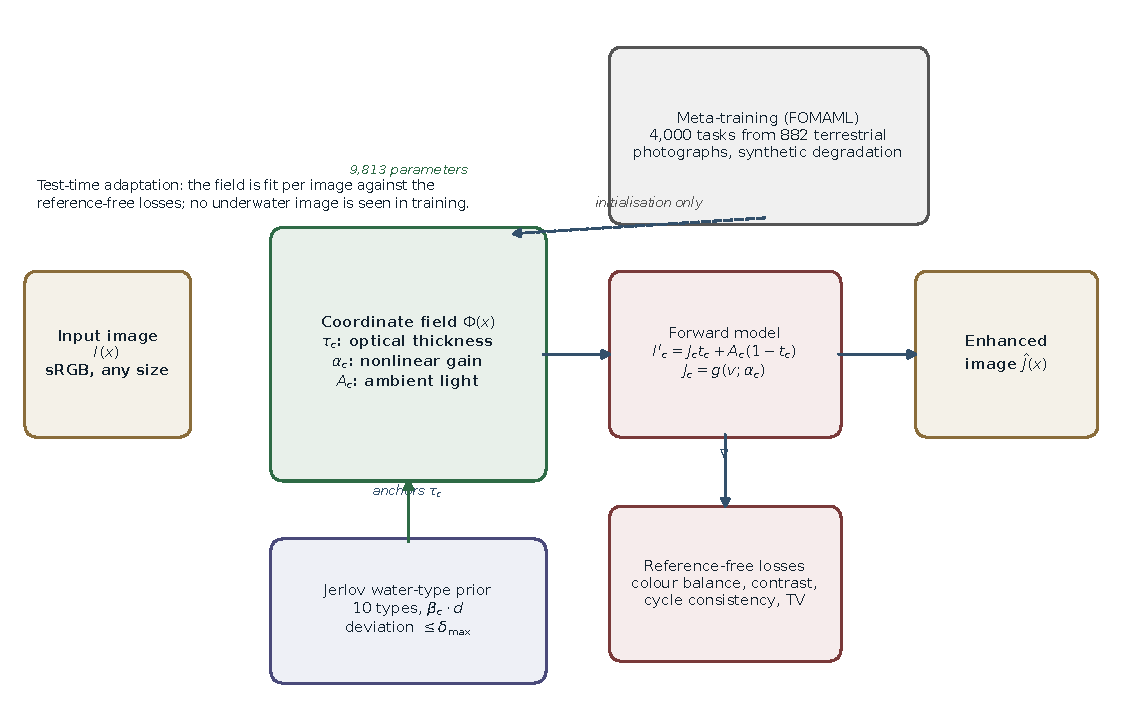
\includegraphics[width=\columnwidth]{figures/method_diagram.pdf}
\caption{The PhysINR-Zero pipeline: forward model, coordinate field, meta-initialisation and per-image adaptation.\label{fig:method}}
\end{figure}

\begin{figure}[!t]
\centering
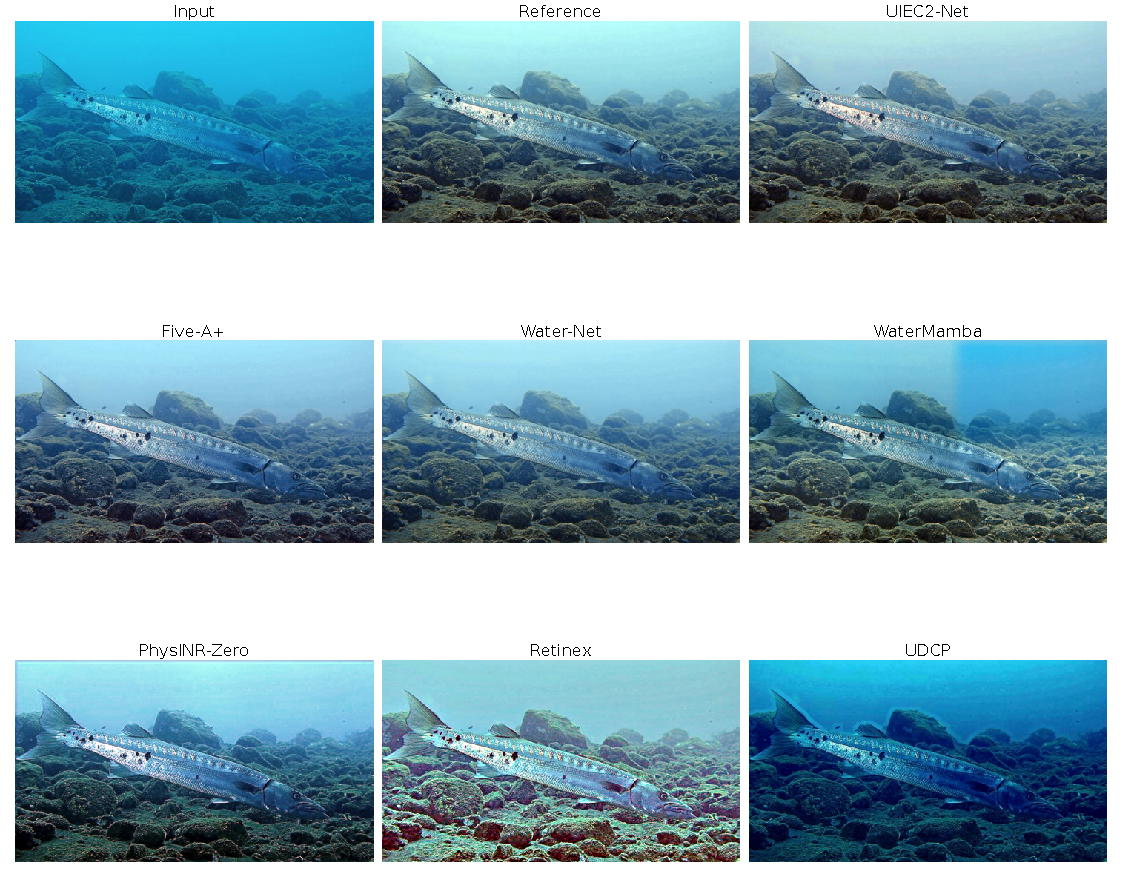
\includegraphics[width=\columnwidth]{figures/qualitative_UIEB.pdf}
\caption{Representative UIEB test frame: input, PhysINR-Zero, and the supervised networks that lead the paired metrics.\label{fig:qualitative}}
\end{figure}

\begin{figure}[!t]
\centering
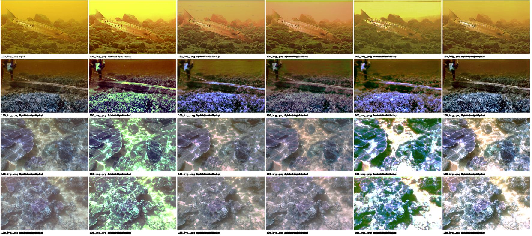
\includegraphics[width=0.49\textwidth]{figures/revision_v4_uieb.pdf}
\vspace{2pt}
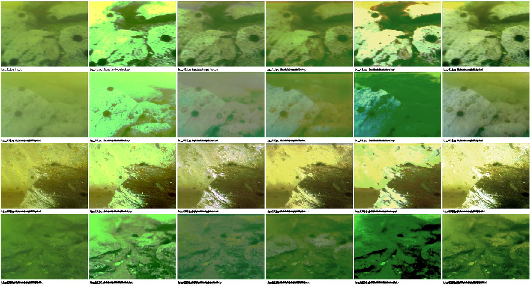
\includegraphics[width=0.49\textwidth]{figures/revision_v4_uccs.pdf}
\caption{Prior design study frames (Section 4.4): the legacy lookup (A), the measured-only prior (B), the uncalibrated (C) and calibrated (D) level heads against input and reference.\label{fig:revision}}
\end{figure}

\begin{figure*}[!t]
\centering
\begin{tabular}{cc}
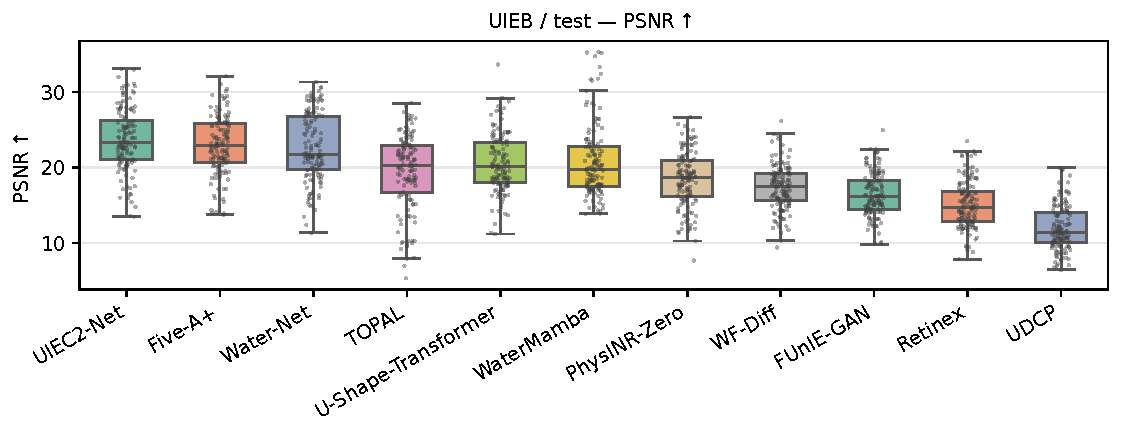
\includegraphics[width=0.49\columnwidth]{figures/box_UIEB_psnr.pdf} & 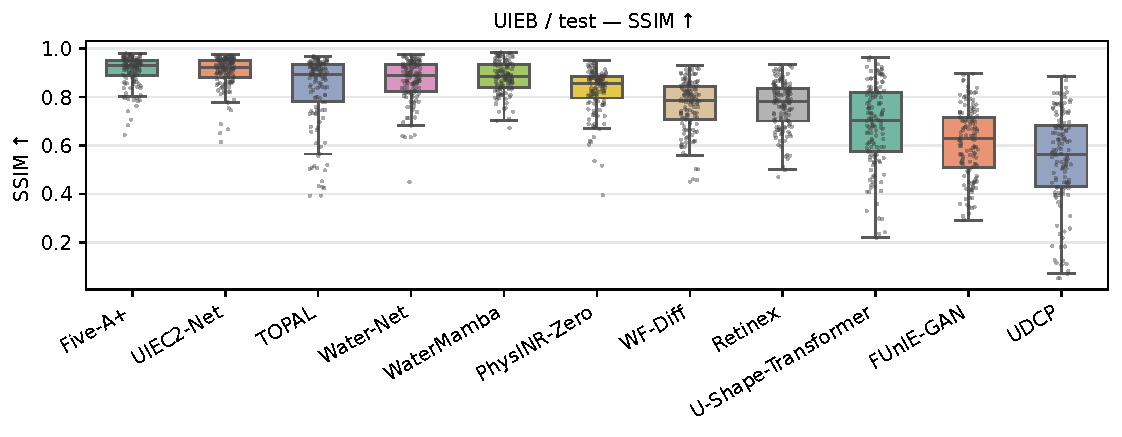
\includegraphics[width=0.49\columnwidth]{figures/box_UIEB_ssim.pdf} \\
\vspace{2pt} & \vspace{2pt} \\
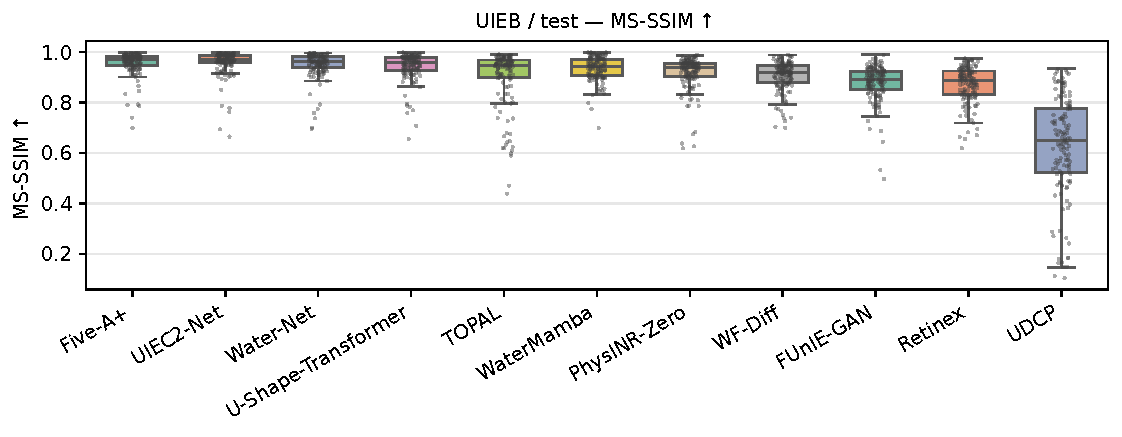
\includegraphics[width=0.49\columnwidth]{figures/box_UIEB_ms_ssim.pdf} & 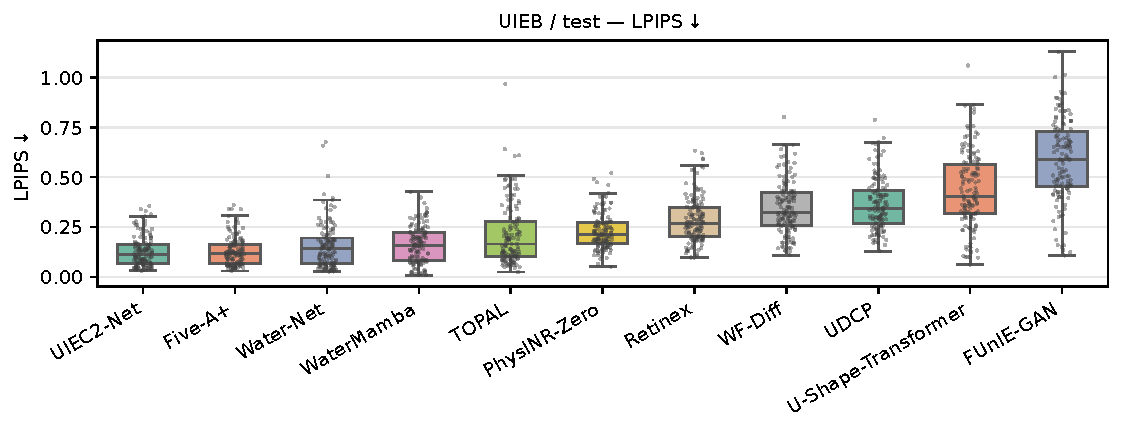
\includegraphics[width=0.49\columnwidth]{figures/box_UIEB_lpips_alex.pdf} \\
\end{tabular}
\caption{UIEB score distributions (PSNR, SSIM, MS-SSIM, LPIPS-AlexNet) for all eleven methods.\label{fig:box-uieb}}
\end{figure*}

\begin{figure}[!t]
\centering
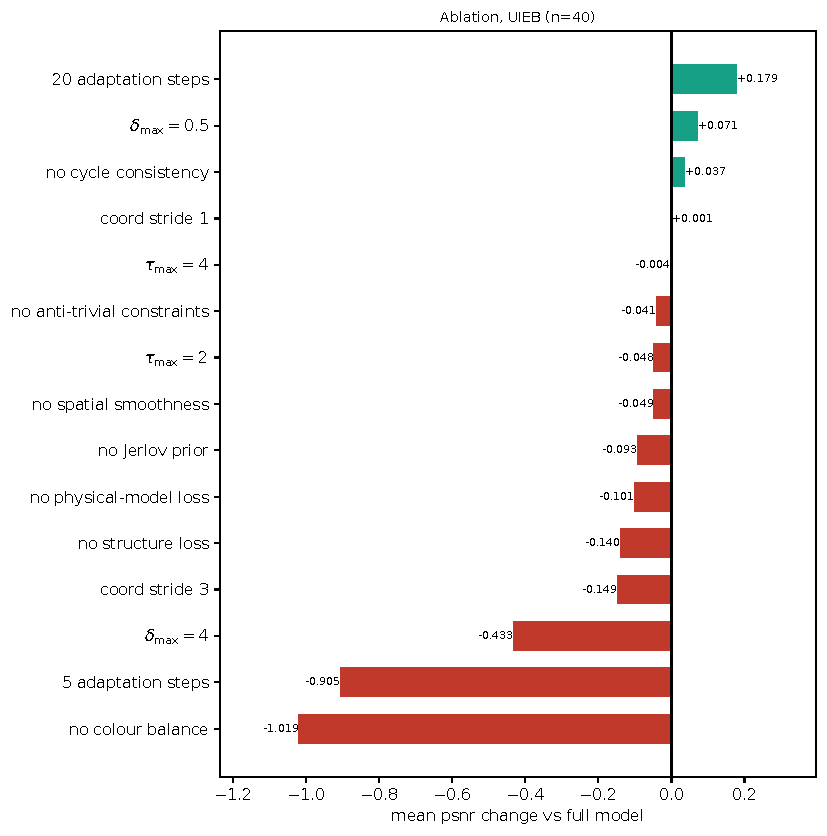
\includegraphics[width=\columnwidth]{figures/ablation_UIEB_psnr.pdf}
\caption{Ablation PSNR distributions on the 40-image UIEB subset.\label{fig:ablation}}
\end{figure}

\section*{Acknowledgment}

\paragraph*{Use of artificial intelligence}
The authors disclose the use of an AI assistant (ZCode, Atria model) during
the preparation of this manuscript. The assistant was used for drafting and
editing prose, consolidating bibliographic records, and developing the
benchmark code under the direction of the authors. All scientific content,
experimental design, results and conclusions were produced and verified by
the authors, who take full responsibility for the work.

\paragraph*{Data availability}
All five benchmark datasets are publicly available: UIEB~\cite{li2020uieb},
LSUI~\cite{peng2023ushape}, EUVP~\cite{islam2020funie},
RUIE/UCCS~\cite{ruiedataset}, and the DIV2K photographic
pool~\cite{agustsson2017ntire} used for meta-training. Code, per-image
results, provenance records and the trained checkpoint are available at
\url{https://github.com/bornaseirco/PhysINR}.

\bibliographystyle{IEEEtran}
\bibliography{references}
\end{document}
